\pdfminorversion=7 % draw.io exports PDF 1.7; allow inclusion
\documentclass[sigconf,nonacm]{acmart}

% acmart already defines \Bbbk; amssymb redefining it is an error, not a warning.
\let\Bbbk\relax
\usepackage{amsmath,amssymb,amsfonts,latexsym}
\usepackage{enumerate}
\usepackage{xspace}
\usepackage{colortbl,multirow,hhline}
\usepackage{listings}
\usepackage{caption}
\usepackage[normalem]{ulem}
\usepackage{xcolor}
\usepackage{pifont}
\usepackage{url}
\usepackage{balance}
\usepackage{graphicx}
\usepackage{longtable}
\usepackage{booktabs}
\usepackage{enumitem}
\usepackage{array}

% Keep the expanded, source-complete bibliography on the report's final page.
\renewcommand{\bibfont}{\scriptsize}

\renewcommand{\ttdefault}{cmr}

\newcommand{\todo}[1]{\textcolor{blue}{\ding{46}~#1}}
\newcommand{\ie}{\emph{i.e.,}\xspace}
\newcommand{\eg}{\emph{e.g.,}\xspace}
\newcommand{\etc}{etc.\xspace}
\newcommand{\etal}{\emph{et~al.}\xspace}

\acmYear{2026}
\settopmatter{printacmref=false}
\acmConference[S2 Project '26]{Research Project — Software and Sustainability (S2) Group}{June--September, 2026}{Vrije Universiteit Amsterdam, The Netherlands}

\begin{document}

\title[Self-Hosted LLMs under an Agentic AutoML Workload]{
	Evaluating Self-Hosted LLM Architectures under an Agentic AutoML Workload: An Energy/Accuracy Pareto Study of \texttt{autoresearch}
}
\subtitle{Research Project Report --- 6 ECTS}

\author{Houcen Liu}
\affiliation{%
 \institution{Vrije Universiteit Amsterdam}
 \city{Amsterdam}
 \country{The Netherlands}
} \email{houcenliu@gmail.com}

\begin{abstract}
\noindent \textit{Context}.
Self-hosting large language models promises privacy, cost control, and independence from frontier-API providers, but its viability hinges on whether locally-served models deliver acceptable accuracy at acceptable energy cost on realistic workloads. Agentic loops, in which an LLM repeatedly proposes, evaluates, and revises actions, are among the most demanding and least-measured of such workloads.

\noindent \textit{Goal}.
We evaluate whether a simple self-hostable model architecture, a sparse Mixture-of-Experts (MoE) model compared against a dense model of the same family, can drive an agentic AutoML loop with good performance and energy efficiency, and we identify the intra-model and agent-loop configurations that improve on the baseline energy/accuracy profile. Karpathy's \texttt{autoresearch} is the case-study workload.

\noindent \textit{Method}.
A controlled experiment following the Green Lab methodology combines a $2 \times 2 \times 2$ full-factorial Phase~1 design (proposer architecture $\times$ patience $\times$ loop budget) with 3 repetitions (24 sessions, 360 iterations) and three exploratory follow-ups on reasoning and sampling temperature (30 sessions, 300 iterations). Training and proposer inference run on separate RTX 4000 Ada GPUs. NVML provides gross session-level GPU-board measurements, while timestamps attribute iteration windows; raw EnergiBridge traces permit a post-hoc sensitivity analysis that adds AMD CPU-package energy. The planned CPU-served proposer phase is not part of the present results while its scope awaits supervisor feedback.

\noindent \textit{Results}.
The sparse proposer used 42.0\,\% less GPU-board energy per session
(90.7 vs.\ 156.4\,kJ; ART-ANOVA $p = 7\times10^{-6}$, partial $\eta^2 = 0.73$).
Adding the recoverable CPU-package counter gives the same conclusion at a broader
measurement scope (179.8 vs.\ 294.5\,kJ, $-39.0\,\%$), but is not a full-system
estimate because DRAM and other host components were not measured. Mean test
accuracy was 2.85 percentage points higher for the MoE (0.8224 vs.\ 0.7939), but
the 95\,\% interval includes zero ($p=0.053$; HC3 sensitivity $p=0.098$), so
accuracy superiority is not established. The MoE retained 17 improvements against
12 and had one no-progress session against five. Correctly pooling all sessions,
including zero-kept sessions, gives 64.0 vs.\ 156.4\,kJ of GPU energy per retained
improvement ($-59.1\,\%$); doubling the loop budget raises that quantity by
146.2\,\%. Of total Phase-1 GPU energy, 78.1\,\% is attributable to non-retained
iterations, 8.2\,\% to retained iterations, and 13.6\,\% remains outside aligned
iteration windows.

\noindent \textit{Conclusions}.
On this workload and hardware, sparsity provides a large energy
advantage and a higher observed mean accuracy, but evidence about the accuracy
contrast is inconclusive; neither superiority nor equivalence is established. Reasoning increases energy in both
arms and shows an exploratory architecture-by-reasoning accuracy interaction.
Sampling temperature clearly changes exact proposal duplication, but the outcome
experiments are too small, and confounded with a prompt change at restart, to
establish that temperature does not affect retention or accuracy. A keep threshold
must be derived from a measured noise floor. A 100-iteration MoE session and
retained-checkpoint replay are prepared as the next extension but are not reported
as completed evidence.
\end{abstract}

\maketitle

\section{Introduction}

Large language models are increasingly consumed as remote frontier APIs, yet a growing community of users, researchers, and practitioners wants to \emph{self-host}: running open-weight models on hardware they own, for privacy, cost predictability, reproducibility, and independence from providers. The open question is not whether self-hosting is possible (mature serving stacks and quantized open weights make it routine) but whether it is \emph{viable}: does a self-hosted model deliver acceptable task accuracy at acceptable energy cost on the workloads people actually run? Energy is central to this question. The environmental footprint of ML is well documented at the training end \cite{schwartz2020green} and, more recently, at the inference end \cite{luccioni2024power}, and the software engineering community has called for empirical, measurement-driven approaches to Green AI \cite{cruz2024innovating}. However, published inference-energy figures overwhelmingly come from single-prompt benchmarks. They say little about \emph{agentic} workloads, in which an LLM is invoked hundreds of times inside a feedback loop, interleaved with other computation, and where a poorly steering model wastes its own inference joules and the joules of every downstream computation it triggers.

Agentic AutoML is a sharp instance of this workload class, and a deliberately chosen one: unlike open-ended agentic systems it has fixed-length inner experiments, a binary per-iteration outcome, and a ground-truth accuracy signal that is independent of the agent's own judgment. Those three properties are what make energy attributable to a phase and success measurable without a human oracle, most agentic workloads offer none of them. In Karpathy's \texttt{autoresearch} \cite{karpathy2026autoresearch}, an LLM \emph{proposer} iteratively mutates the training recipe of an inner machine-learning workload, launches a short training experiment for each mutation, inspects the outcome, and decides to keep or revert the change; in this study the inner workload is a compact convolutional network trained on CIFAR-10. A single session comprises tens of iterations, each combining LLM inference with a fixed, short burst of GPU training (45\,s here, set by calibration). The total energy cost of a session therefore depends jointly on (i) the proposer's architecture and serving configuration and (ii) the agent-loop configuration that governs how many experiments are run and how failures are handled. No published energy evaluation of \texttt{autoresearch}, or of any comparable agentic AutoML loop, exists to date.

This project evaluates a simple self-hostable model architecture under this workload. The architectural contrast is sparse versus dense: \texttt{Qwen3-30B-A3B}, a Mixture-of-Experts model holding 30.5B parameters but activating only $\sim$3B per token, against \texttt{Qwen3-14B}, a dense model from the same family, both quantized to int4 with AWQ and both fitting a single 20\,GB card. MoE sparsity is precisely the kind of ``simple architecture'' that could make self-hosting attractive, promising large-model quality at small-model inference cost; whether the theoretical per-token savings survive contact with a real agentic workload, and whether they cost final task accuracy, is an empirical question. Alongside the architectural factor we sweep two agent-loop configurations, \emph{patience} (how many consecutive regressions the agent tolerates before reverting) and \emph{loop budget} (the maximum number of inner experiments per session), each with a registered energy-relevance hypothesis.

Importantly, \texttt{autoresearch} is used here as a \emph{case study}, not as an object of scientific assessment: we evaluate its characteristics as a workload (single-machine, instrumentable, with a built-in ground-truth accuracy signal) and make no claims about the quality of the research it automates. The experiment is conducted according to the guidelines of Wohlin \etal \cite{wohlin12}, using the S2 group's \texttt{experiment-runner} framework \cite{karsten2025experimentrunner} as a session-level orchestrator, with \texttt{EnergiBridge} \cite{sallou2023energibridge} for energy measurement. The agent loop itself is re-implemented rather than adopted: the upstream repository publishes the protocol but no runnable loop, and, more importantly, the experiment requires loop policy to be \emph{enforced} rather than prompted and phase boundaries sharp enough to cut a power trace on (Section~\ref{sec:execution}). Because training and proposer inference are placed on physically separate GPUs, per-component energy is measured directly rather than estimated. A second experimental phase re-runs a subset of configurations with the proposer served on CPU only, for the self-hoster without a GPU.

From the results, practitioners will learn (i) whether an MoE architecture buys real energy savings on agentic workloads without losing accuracy, (ii) which agent-loop configurations sit on the energy/accuracy Pareto frontier, readable as direct configuration guidance (``at energy budget $X$, the most accurate configuration is $Y$''), and (iii) whether CPU-only proposer serving is a tolerable fallback. Researchers gain a reusable measurement pattern, session-level orchestration with per-device energy attribution, an error taxonomy that separates infrastructure failure from agent failure, and a keep threshold derived from a measured noise floor rather than assumed, together with a full replication package.

\section{Background}\label{sec:background}

This section introduces the concepts the experiment builds on, for readers outside the LLM-systems niche.

\textbf{Self-hosting LLMs.} Open-weight models (\eg the Qwen, Llama, Gemma, and Granite families) can be downloaded and served on hardware the user controls, instead of being consumed through a provider's API. Self-hosting trades the convenience and raw capability of frontier APIs for privacy (data never leaves the machine), cost predictability, reproducibility (pinned weights, no silent model updates), and independence. Its practical viability depends on whether a locally-served model is accurate \emph{enough} and cheap \emph{enough} on the user's actual workload, in energy as well as in money.

\textbf{Dense vs.\ Mixture-of-Experts architectures.} In a \emph{dense} transformer, every parameter participates in every token's computation, so inference cost grows with total model size. A \emph{Mixture-of-Experts} (MoE) model replaces feed-forward blocks with many parallel ``experts'' of which a router activates only a few per token: \texttt{Qwen3-30B-A3B} holds 30.5B parameters but activates only $\sim$3B per token. MoE thus promises large-model quality at small-model per-token compute, an attractive proposition for self-hosting, where the energy budget is the user's own. Whether the promise holds on a real agentic workload, where proposal \emph{quality} feeds back into downstream compute, is this experiment's architectural question.

\textbf{Quantization and intra-model configuration.} Model weights are typically released at 16-bit precision; \emph{quantization} compresses them to lower precision (here int4, $\sim$4 bits per weight), shrinking memory and energy per token at some accuracy risk. Quantization level, sampling temperature, context handling, and serving-stack settings together form the model's \emph{intra-model configuration}. In this experiment the intra-model configuration is deliberately \emph{fixed} (AWQ int4, temperature 0.7, reasoning disabled) so that Stage~1 isolates the architectural effect; varying these settings for further optimization is Stage~2 of the staged design (Section~\ref{sec:planning}).

\textbf{Agentic loops and \texttt{autoresearch}.} An \emph{agentic} workload invokes an LLM repeatedly inside a feedback loop rather than once per user prompt. Karpathy's \texttt{autoresearch} \cite{karpathy2026autoresearch} is an agentic AutoML system whose iteration cycle is shown in Figure~\ref{fig:autoresearch-loop}. Each iteration starts from \texttt{program.md}, a Markdown file holding the task description, the current training recipe of the inner workload, and the history of past attempts. The LLM \emph{proposer} reads this state and proposes a \emph{mutation}: a concrete diff to the recipe (\eg a hyperparameter change, an architectural tweak, a data-pipeline edit). The mutated recipe is trained for a bounded, fixed-time experiment. In this study the inner workload is a compact convolutional network on CIFAR-10; \texttt{autoresearch}'s default inner workload is \texttt{nanochat}, a small LLM training pipeline, and the swap (motivated by the schedule, Section~\ref{sec:execution}) preserves the protocol's semantics. The resulting checkpoint is scored by validation accuracy (\texttt{val\_acc}) on a held-out split. A mutation becomes the new best only when \texttt{val\_acc} exceeds the previous best by more than the measured threshold $\epsilon$. A below-threshold mutation is retained \emph{provisionally} as context for the next proposal; a later new best absorbs that chain, whereas reaching the configured \emph{patience} rolls the whole provisional chain back to the best recipe. The loop repeats until the session's \emph{loop budget} (maximum number of outer-loop attempts) is exhausted; internal proposer retries stay within one attempt. Guard rejection, proposer error, and training error consume attempts and are logged without becoming retained mutations. At exhaustion, any pending provisional chain is rolled back and the best checkpoint is evaluated once on the CIFAR-10 test set. Each attempt records its outcome and available token and timing metadata in the session log that this experiment parses for its dependent variables. A session therefore interleaves many LLM inferences with many short, fixed-length GPU training runs, and total energy depends jointly on the proposer and on the loop's configuration; this is why both appear as factors in this study. Validation accuracy and test-set accuracy serve as the ground-truth accuracy metrics.

\begin{figure}[htbp]
\centering
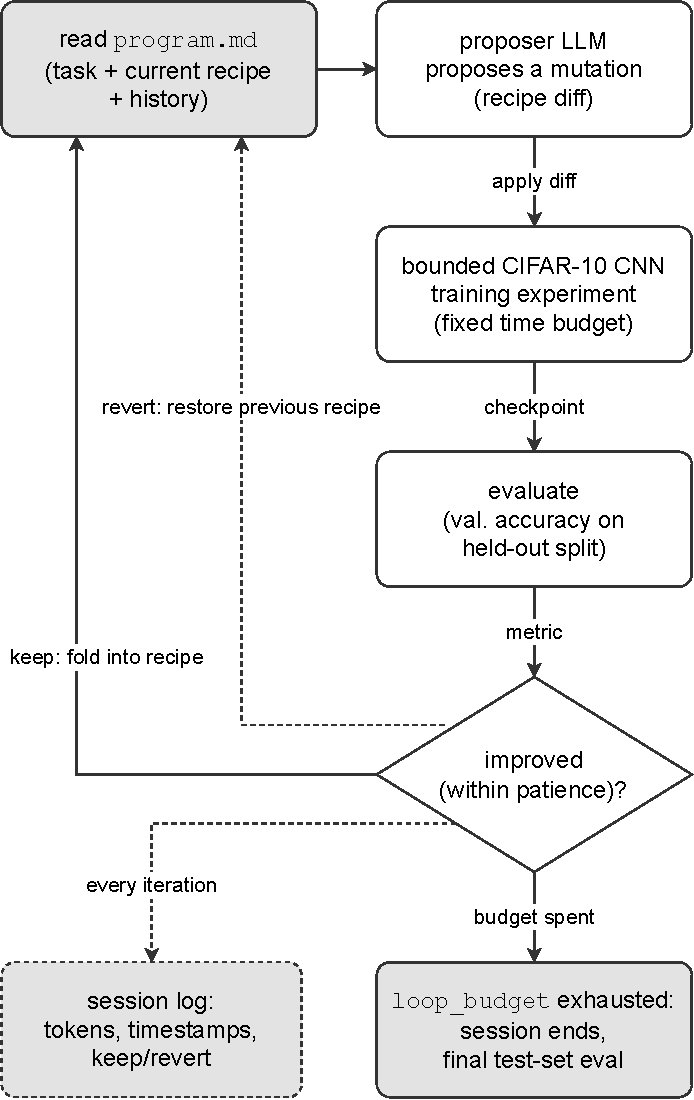
\includegraphics[width=\columnwidth]{figures/autoresearch_loop.drawio.pdf}
\caption{The implemented \texttt{autoresearch} loop. Every scheduled outer-loop attempt consumes
the fixed loop budget, including proposer error, guard rejection, and training error. A valid
candidate is kept only when \texttt{val\_acc} exceeds the best score by more than
$\epsilon$; otherwise a valid below-threshold candidate remains provisional until a later keep absorbs the chain,
or patience or budget exhaustion rolls it back. At budget exhaustion, the best
checkpoint is evaluated once on the test split.}
\Description{Flowchart showing mutation proposal, proposer and guard failures, bounded training, training error, epsilon-qualified keep, provisional retention, patience rollback, fixed-budget accounting, and final rollback plus one test evaluation.}
\label{fig:autoresearch-loop}
\end{figure}

\textbf{Energy measurement.} Modern hardware exposes energy and power counters. NVIDIA's NVML \cite{nvidia2026nvml} reports board power per GPU; the AMD host used here exposes a CPU-package energy counter through \texttt{EnergiBridge} \cite{sallou2023energibridge}. The archived trace does not contain a separate DRAM counter. Integrating or differencing these counters over the same timestamp bounds yields energy for the measured components in joules, but not wall-power or full-system energy. Because NVML is per-GPU, placing training and proposing on separate devices provides a useful device-associated decomposition, while still including each device's idle and weight-residency draw. The \texttt{experiment-runner} framework \cite{karsten2025experimentrunner} automates the surrounding protocol: run tables, factor randomization, instrumentation lifecycle, and result collection.

\section{Related Work}\label{sec:related}

Karsten \etal present \texttt{experiment-runner} \cite{karsten2025experimentrunner}, the S2 group's framework for orchestrating measurement-based experiments on software systems; it defines run tables, factor sweeps, and lifecycle hooks for instrumentation. Our experiment uses the framework in a configuration not previously reported: as a \emph{session-level} orchestrator, where one ``run'' is a complete agent session of 15--40 minutes rather than a short deterministic program invocation. Two small changes to the vendored framework were required and are documented in the replication package: the profiler launches the target program as its own child, so the target's working directory, environment and output redirection had to be made settable (without this the measured program can fail to start while the profiler records a perfectly valid trace of an idle machine), and the profiler's assumption that raised privileges are always needed for RAPL had to become configurable, since they are not needed on our host.

Sallou \etal introduce \texttt{EnergiBridge} \cite{sallou2023energibridge}, a cross-platform energy profiler sampling CPU (RAPL) and GPU (NVML) power. We adopt the tool itself unchanged; our contribution on the measurement side is the per-GPU attribution design, which places proposer inference and inner-loop training on physically separate devices so that NVML readings decompose session energy without modeling assumptions, together with the alignment gate that verifies the decomposition empirically (during training the training device must draw substantially more than the proposer device, and the reverse while proposing) rather than assuming the device indices are wired correctly.

Cruz \etal \cite{cruz2024innovating} position the convergence of software engineering and Green AI and explicitly name complex, composite AI workloads as underserved measurement targets. Our experiment answers that call for the agentic AutoML class, which their agenda anticipates but does not measure.

Cursaru \etal \cite{cursaru2024codellama} run a controlled experiment on the energy efficiency of Code Llama-generated source code, using the same GQM and factorial-design tradition. Their unit of analysis is the generated artifact; ours is the generating loop itself: we measure the energy of the agentic process, not of its outputs.

Lu \etal's AI Scientist \cite{lu2024aiscientist} and its successor \cite{yamada2025aiscientist2} automate the full research pipeline end-to-end. They are the most prominent agentic-research systems but are poorly suited to controlled energy measurement: multi-hour heavy-tailed sessions, fuzzy success oracles, and high per-run API cost. Beel \etal's critical evaluation \cite{beel2025evaluating} documents these failure modes. We instead select \texttt{autoresearch}, whose fixed-length inner experiments and binary keep/revert outcomes make it tractable as a measurement case study; our interest is the workload's energy characteristics, not the scientific quality of its outputs.

Huang \etal's MLAgentBench \cite{huang2024mlagentbench} benchmarks LLM agents on ML experimentation tasks and measures success rates and API cost. Energy is absent from their evaluation; we treat it as a first-class dependent variable and relate it to ground-truth accuracy rather than to task-completion counts.

Krupp \etal \cite{krupp2026webagents} provide a recent empirical energy benchmark of web agents across open models and GPUs. Their work establishes agent-level energy measurement as an emerging line of research, but studies web-navigation episodes and task success rather than a closed propose--train--evaluate--keep AutoML loop. It is therefore the closest agentic-energy precedent we found, not a like-for-like comparator.

Luccioni \etal \cite{luccioni2024power} measure inference energy across model architectures and tasks and establish that per-inference cost varies by orders of magnitude with architecture; this is the single-prompt analogue of our proposer factor. Our experiment extends this line from isolated prompts to a fixed-budget agentic loop, where proposer quality changes retained yield and energy per retained change.

\subsection{How our results compare}

Because our literature review (cut off in August~2026) found no directly
comparable energy measurement of a propose--evaluate--keep AutoML loop, our
headline numbers cannot be compared like for like. Three partial comparisons
are possible.

Luccioni \etal \cite{luccioni2024power} find per-inference energy varying by
orders of magnitude with architecture on single prompts. Our proposer-phase
measurements are consistent in direction but far smaller in spread: a
2.6$\times$ difference between a 30B sparse and a 14B dense model at equal
quantization on one card. The gap is expected, their range spans model classes
and task types, ours holds everything but sparsity fixed, but it suggests
single-prompt figures should not be extrapolated to closed loops, where our
$E_{\mathit{GPU1}}$ is only 40--60\,\% of session GPU energy. Under the fixed
10- or 20-iteration budgets used here, proposal quality governs retained yield
rather than the number of planned training runs.

MLAgentBench \cite{huang2024mlagentbench} reports agent success rates on ML
experimentation tasks and treats API cost as the resource. Our contract-compliance
result complicates that accounting: the arm with the \emph{higher} rejection rate
(9.6\,\% vs.\ 0.0\,\%) produced the better recipes, so a benchmark scoring
well-formed output would have ranked our two subjects in the wrong order. We would
expect the same dissociation to affect success-rate metrics that require parseable
agent actions.

Cursaru \etal \cite{cursaru2024codellama} measure the energy of code an LLM
generates. Our unit is the generating loop rather than its output, and the two
compose: in our sessions 78.1\,\% of GPU energy was attributable to iterations
whose mutations were not retained, 8.2\,\% to retained iterations, and 13.6\,\%
fell outside aligned iteration windows. A study of generated-code efficiency sees
only part of this loop-level accounting.

\section{Experiment Definition}\label{sec:definition}

Following the Goal--Question--Metric template \cite{wohlin12}, the goal of this experiment is:

\begin{quote}
\textbf{Analyze} self-hosted LLM proposer architectures and agent-loop configurations\\
\textbf{for the purpose of} evaluation\\
\textbf{with respect to} their energy efficiency and task accuracy\\
\textbf{from the point of view of} researchers and practitioners who want to self-host LLMs\\
\textbf{in the context of} the \texttt{autoresearch} agentic AutoML loop running on self-hosted (GPU and CPU-only) hardware.
\end{quote}

The goal refines into two research questions:

\begin{description}[leftmargin=1.2em]
\item[RQ1.] \emph{How do agent-loop configuration choices move the energy/accuracy profile of \texttt{autoresearch}?}
\item[RQ2.] \emph{Which configurations sit on the energy/accuracy Pareto frontier?}
\end{description}

RQ1 is analytic: it quantifies the main and interaction effects of proposer architecture, patience, and loop budget on session energy and final accuracy, together with the mechanistic decomposition (proposer vs.\ training energy, energy wasted on reverted mutations). RQ2 is synthetic: it aggregates the same measurements into a Pareto frontier over (total session energy, final accuracy) and reads off the non-dominated configurations, including the designated baseline cell against which improvements are reported. The CPU-only phase re-evaluates a subset of frontier cells to test whether the frontier survives GPU-less proposer serving.

\begin{figure}[htbp]
\centering
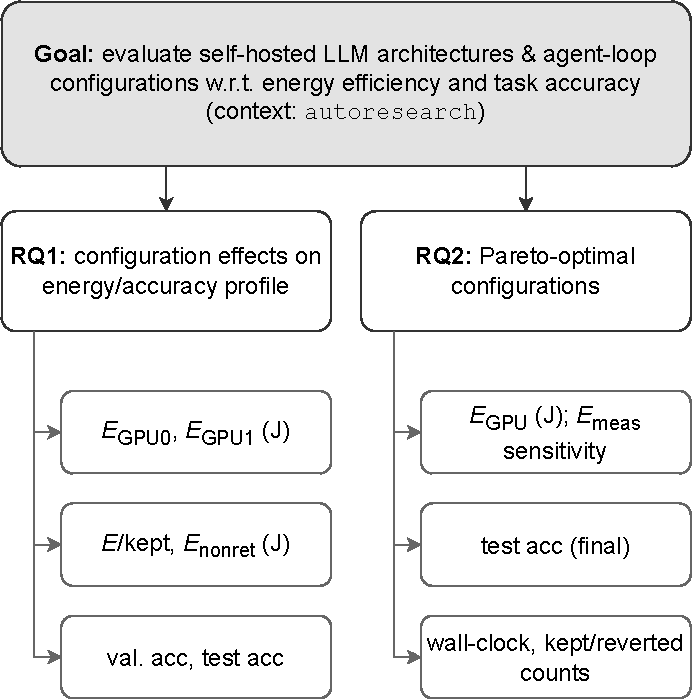
\includegraphics[width=\columnwidth]{figures/gqm.drawio.pdf}
\caption{GQM tree: goal, research questions, and metrics.}
\label{fig:gqm}
\end{figure}

Figure~\ref{fig:gqm} maps the goal to questions and metrics. All energy metrics are direct measurements (RAPL/NVML via \texttt{EnergiBridge}); accuracy metrics are ground-truth workload outcomes (validation accuracy during the loop and CIFAR-10 test-set accuracy at session end), deliberately distinct from the agent's own keep/revert judgments, which this experiment treats as behavioral signals rather than accuracy measures.

\section{Experiment Planning}\label{sec:planning}

\subsection{Subjects Selection}

The \emph{system under evaluation} is the self-hosted LLM proposer. Two subjects are selected from the same model family and training recipe, isolating the architectural contrast of interest:

\begin{itemize}[leftmargin=1.2em]
\item \texttt{Qwen/Qwen3-14B-AWQ}: dense, 14.8B parameters, 9.3\,GiB at int4;
\item \texttt{QuixiAI/Qwen3-30B-A3B-AWQ}: Mixture-of-Experts, 30.5B total with $\sim$3B active per token, 15.6\,GiB at int4.
\end{itemize}

\textbf{Deviation from the originally proposed pair.} The Qwen3.6 models named in an earlier draft cannot be served on a 20\,GB card: both exceed it \emph{on weights alone}, before any KV cache (27B AWQ = 19.05\,GiB; 35B-A3B AWQ $\approx$ 22.4\,GiB). The cause is that Qwen3.6 is multimodal and the quantizer leaves the vision tower, \texttt{lm\_head} and the linear-attention projections at 16 bits: the Hub metadata reports \texttt{I32: 25.47B, F16: 3.33B, BF16: 0.52B}, i.e.\ 3.85B unquantized parameters ($\approx$7.7\,GB) on top of 12.7\,GB of int4 weights. ``27B at int4'' does not imply 13.5\,GB. Qwen3-32B-AWQ was evaluated and rejected on arithmetic: 18.0\,GiB of weights plus $\approx$0.8\,GiB of fp8 KV cache and $\approx$1.1\,GiB of CUDA context and activations totals $\approx$19.9\,GiB against a 19.99\,GiB card.

The replacement pair fits comfortably and arguably sharpens the research question: given one 20\,GB GPU, does a 30B sparse model activating $\sim$3B parameters per token outperform a 14B dense model activating all of them? That is the decision a self-hoster actually faces. Two limitations follow and are carried into Section~\ref{sec:threats}: no single publisher ships AWQ builds of both models, so the dense arm is Qwen's official quantization and the MoE a third-party build of the same method and bit-width; and total capacity is unequal (30.5B vs.\ 14.8B), so sparsity and capacity are not fully separable. Both repositories and exact revisions are recorded in the run-table metadata. The pre-registered backup pair (IBM Granite~4.1 8B vs.\ 30B) was not needed.

The \emph{case-study workload} is the \texttt{autoresearch} protocol \cite{karpathy2026autoresearch}, a single editable training file, a fixed wall-clock budget per experiment, one scalar metric, and a keep-or-revert decision, driving the training of a compact convolutional network on CIFAR-10 at a per-experiment budget set by calibration to \textbf{45\,s} (Section~\ref{sec:execution}). The upstream repository publishes the protocol and its default inner workload but not a runnable agent loop, so the loop was re-implemented for this experiment; Section~\ref{sec:execution} explains why a purpose-built loop is required for the measurement rather than merely convenient. \texttt{autoresearch} ships with \texttt{nanochat}, a small LLM training pipeline, as its default inner workload; this study substitutes the CNN and preserves the protocol's semantics. The reason is schedule: \texttt{nanochat} costs 25--35 min per inner experiment on this hardware, which does not fit the compressed 4-week timeline, while the CNN keeps the full factorial affordable. \texttt{autoresearch} is selected for its workload characteristics (single-machine operation, fixed-length inner experiments, per-iteration keep/revert outcomes, and clean ground-truth evaluation metrics), not for the quality of the research it automates, which is out of scope. The \texttt{nanochat} workload is kept as a specified extension (Section~\ref{sec:conclusions}).

\subsection{Experimental Variables}

\begin{table}[htbp]
\caption{Independent variables (factors).}
\label{tab:factors}
\small
\begin{tabular}{@{}p{1.7cm}p{1.9cm}p{2.8cm}@{}}
\toprule
\textbf{Factor} & \textbf{Levels} & \textbf{Rationale} \\
\midrule
\texttt{proposer} & dense (14B); MoE (30B-A3B) & Architectural contrast: does sparsity buy energy without losing accuracy? \\
\texttt{patience} & greedy; patience-3 & Revert on first regression vs.\ tolerate up to 3 consecutive regressions. \\
\texttt{loop\_budget} & 10; 20 & Max inner experiments per session ($\approx$17\,min / $\approx$32\,min as executed). \\
\bottomrule
\end{tabular}
\end{table}

Table~\ref{tab:factors} lists the three factors, each at two levels. \emph{Fixed variables:} workload (CIFAR-10 CNN, fixed 45\,s training budget), intra-model configuration, namely quantization (int4, AWQ for both arms) and sampling (temperature 0.7, $\mathit{top\text{-}p}$ 0.95; see Section~\ref{sec:threats} for why temperature 0 was abandoned), reasoning mode (disabled for both arms and verified by measurement), hardware assignment (training on GPU~0, proposer on GPU~1, both RTX 4000 Ada), and pinned software versions. Fixing the intra-model configuration is a deliberate consequence of the staged design (Section~\ref{sec:design}): Stage~1 isolates the architectural effect; intra-model settings become factors only in Stage~2.

\begin{table}[htbp]
\caption{Dependent variables.}
\label{tab:depvars}
\small
\begin{tabular}{p{2.6cm}p{5.2cm}}
\toprule
\textbf{Variable} & \textbf{Operationalization} \\
\midrule
$E_{\mathit{GPU}}$ (J) & Primary executed energy outcome: sum of NVML board-energy integrals for GPU~0 and GPU~1 over the session. \\
$E_{\mathit{GPU0}}, E_{\mathit{GPU1}}$ (J) & Whole-session energy of the training and proposer devices, respectively. These are device-associated, not pure phase costs, because each board remains powered throughout. \\
$E_{\mathit{meas}}$ (J) & Sensitivity scope reconstructed from archived traces: $E_{\mathit{GPU}}+E_{\mathit{CPU,pkg}}$. The AMD trace has no separate DRAM counter, so this is not full-system energy. \\
$E/\mathrm{kept}$ (J) & Pooled across sessions in a group: $\sum E / \sum |\{\text{kept}\}|$. Zero-kept sessions contribute energy to the numerator and zero to the denominator; they are never dropped. Scope (GPU or measured components) is stated with each value. \\
$E_{\mathit{nonret}}$ (J) & Phase-aligned GPU energy of reverted, rejected, errored, or rollback-discarded iterations. Unaligned session energy is reported separately rather than silently classified. \\
\texttt{val\_acc} & Validation accuracy on a held-out CIFAR-10 split (continuous, sampled during training). \\
Test accuracy & CIFAR-10 test-set accuracy at session end; ground-truth accuracy, y-axis of the Pareto figure. \\
Wall-clock (s) & Session duration; iterations, kept, reverted, errored counts. \\
\bottomrule
\end{tabular}
\end{table}

Two accuracy-like signals are deliberately kept distinct: the agent's keep/revert decision is its \emph{claim} of improvement (a behavioral variable and the denominator of $E/\mathrm{kept}$), whereas \texttt{val\_acc} and test accuracy are \emph{ground truth} and alone enter the Pareto analysis.

\subsection{Experimental Hypotheses}

One energy-relevance hypothesis is registered per factor (all stated as two-sided nulls; $\mu$ denotes the cell mean of the named dependent variable):

\begin{description}[leftmargin=1.2em]
\item[H$_{0}^{\mathit{prop}}$:] $\mu_{E_{\mathit{GPU}}}$ and $\mu_{\mathrm{acc}}$ (test accuracy) do not differ between dense and MoE proposers. \emph{Mechanism under test:} MoE sparsity can reduce inference energy and latency; with a fixed loop budget, proposer quality changes retained yield and therefore energy productivity rather than the number of scheduled experiments.
\item[H$_{0}^{\mathit{pat}}$:] $\mu_{E_{\mathit{nonret}}}$ and $\mu_{E/\mathrm{kept}}$ do not differ between greedy and patience-3. \emph{Mechanism:} greedy reverts noise quickly (less non-retained energy) but may discard real improvements; patience tolerates regressions longer (more non-retained energy, possibly better final accuracy).
\item[H$_{0}^{\mathit{bud}}$:] $\mu_{E/\mathrm{kept}}$ does not differ between budgets 10 and 20. \emph{Mechanism:} diminishing returns near local optima should raise energy-per-kept-mutation at higher budgets; two levels bound but do not locate the knee.
\end{description}

\subsection{Experiment Design}\label{sec:design}

The design is \emph{staged}: the architecture is studied first, alone, at a fixed intra-model configuration; intra-model settings are varied only afterwards, on the architecture the first stage identifies as preferable. This ordering attributes effects cleanly (architecture first, then configuration headroom) and keeps the factorial tractable.

\textbf{Stage 1, Phase 1 (GPU factorial).} A $2 \times 2 \times 2$ full-factorial design with 3 repetitions: 8 cells, \textbf{24 sessions}, $\approx$10 GPU-hours as executed. Cell execution order is randomized and interleaved across the run table (no blocking by cell), with a \textbf{120\,s} cool-down between sessions for thermal settling; the cool-down was raised from the proposed 60\,s after calibration showed it removes the thermal trend entirely (raw and detrended standard deviations agree to four decimals). Swapping the served model between arms costs 25\,s and occurs outside the measured window. The longest session ran 39\,min. The designated baseline cell is \emph{dense $\times$ greedy $\times$ budget 10}.

\textbf{Planned CPU-served proposer phase (pending).} The proposal specified re-running four frontier-adjacent cells at two repetitions with only proposer inference moved to CPU and training unchanged on GPU~0. This phase has not been executed while its scope awaits supervisor feedback. It is therefore a planned extension, not evidence in the present report, and should not be described as a fully CPU-only loop.

\textbf{Exploratory follow-ups.} Three completed follow-ups vary reasoning mode on both architectures (Stage~2a, 12 sessions), temperature on the MoE (Stage~2b, 12 sessions), and temperature on the dense model (Stage~2c, 6 sessions). Their $n=3$ cells support manipulation checks and exploratory effect estimates, not confirmatory equivalence claims. The originally envisaged quantization and serving-stack sweep was not executed.

Across the completed campaign, 54 valid sessions contribute 660 iterations. A separate 100-iteration MoE session and retained-checkpoint replay are prepared but not yet part of the evidence.

\subsection{Data Analysis}

Analysis proceeds in four steps. (i) \emph{Descriptive statistics}: per-cell means, medians and dispersion for all dependent variables. (ii) \emph{Measurement diagnostics}: GPU energy is plotted against duration and run-table position. The ratio of arm-mean energy to arm-mean duration is used for a transparent average-power decomposition; regression slopes are reported separately. (iii) \emph{Hypothesis testing}: Shapiro--Wilk and Levene diagnostics precede the registered ART-ANOVA for GPU energy. Test accuracy is analyzed at the session level with the same main and two-way factorial terms; effect estimates and 95\,\% intervals are reported because $n=3$ per cell leaves modest accuracy power. The Stage~2a reasoning analysis uses a session-level $2\times2$ model with HC3 intervals and is explicitly exploratory. Corrected energy-per-kept estimates are ratios of pooled sums, with stratified-within-cell bootstrap intervals; zero-kept sessions remain in every numerator. (iv) \emph{Pareto analysis} (RQ2): the non-dominated set over ($E_{\mathit{GPU}}$, test accuracy) across cell means. The keep threshold is a within-session validation decision rule, not an equivalence margin for between-cell test means, so frontier membership is treated as sample-descriptive and accompanied by uncertainty.

Two choices differ from the Green Lab analysis template. We apply the Aligned Rank Transform \cite{wobbrock2011art} rather than transforming the outcome to normality: ART preserves the factorial structure and leaves the interaction terms interpretable, whereas a normalising transform changes the scale on which effects are additive. And we do not include a random effect for the session, because sessions here are independent units rather than repeated measures on the same subject; a within-subject term would misstate the design.

\section{Experiment Execution}\label{sec:execution}

\textbf{Hardware.} A single S2-group workstation hosts the measured stack. The machine provides \textbf{two RTX 4000 Ada cards (20\,GB each)}; GPU~0 runs the inner CNN training and GPU~1 serves the proposer at int4. Idle draw was recorded in experiment notes as 8.63\,W (GPU~0) and 7.90\,W (GPU~1), but the underlying idle traces were not preserved. No idle subtraction is therefore applied: all reported energies are gross over the session boundary and include standby and weight-residency draw. Separate GPUs remove co-location contention and provide direct board-level readings, but whole-session GPU~0/GPU~1 totals are device-associated quantities rather than pure training/proposer phase energy. The CPU-served proposer phase remains pending and is not described as executed.

\textbf{Software infrastructure.} The S2 \texttt{experiment-runner} framework \cite{karsten2025experimentrunner} acts as the \emph{session-level orchestrator}: each run in its run table is one complete \texttt{autoresearch} session. Per run, the runner instantiates the program, selects a proposer endpoint, launches the agent session, and starts two profilers at approximately 10\,Hz: a dedicated NVML sampler for both GPUs and \texttt{EnergiBridge} \cite{sallou2023energibridge} for the host. On this AMD machine the archived EnergiBridge schema exposes one \texttt{CPU\_ENERGY (J)} package counter and no separate DRAM counter. The original parser looked only for Intel-style \texttt{PACKAGE\_ENERGY}/\texttt{DRAM\_ENERGY} columns, leaving \texttt{E\_cpu\_J} blank; CPU-package energy is nevertheless recoverable from the raw trace by differencing the counter over the same session timestamps used for NVML. The registered inferential pipeline therefore remains GPU-only, with measured GPU+CPU-package totals reported as a post-hoc sensitivity analysis. \textbf{Deviation:} the upstream \texttt{autoresearch} repository publishes the protocol and its inner workload but contains no agent loop, so its fixed-budget keep/revert protocol was re-implemented, with patience and loop budget enforced in code. Each Phase-1 archive contains the session log, both raw traces, summary, harness log, and recipe-history bundle. The training-file content record is \texttt{eb632882}; session logs separately record harness repository SHA \texttt{7065bf27}; these identify different artifacts and are not presented as one commit. The two proposer builds are pinned to their HuggingFace revisions (\texttt{Qwen/Qwen3-14B-AWQ} at \texttt{31c69ef}, \texttt{QuixiAI/Qwen3-30B-A3B-AWQ} at \texttt{1ba5586}).

\textbf{Why a purpose-built agent loop.} The upstream \texttt{autoresearch}
repository publishes the protocol and its default inner workload but does not
ship a runnable agent loop, so some implementation was unavoidable. The more
substantive question is why a general-purpose agent framework (Aider, OpenHands,
SWE-agent, AutoGen) was not used instead, since any of them can edit a file in a
loop. Four requirements of this experiment are incompatible with how such
frameworks are built.

\emph{Factors must be enforced, not requested.} Patience and loop budget are
independent variables, so they must mean exactly the same thing for both
proposers. A framework expresses such policy in the prompt and relies on the
model to comply; compliance varies by model, which would confound the factor with
the arm under test. Here both are enforced in Python, so \texttt{patience}~$=3$ is
identical for dense and MoE by construction.

\emph{Iteration attribution needs sharp phase boundaries.} The analysis attributes
iteration-level GPU energy to proposing and training by cutting the 10\,Hz traces
at the instant proposing stops and training starts. The loop
emits \texttt{propose\_start/end} and \texttt{train\_start/end} with paired
wall-clock and monotonic timestamps for exactly this purpose. General agents
interleave tool calls, streaming and internal retries, and expose no such
instant; without it, the decomposition would revert to a modelled estimate, which
is the threat this design exists to avoid.

\emph{Infrastructure failure must be separable from agent failure.} Frameworks
retry internally and absorb the distinction. This experiment depends on it: a
flaky endpoint would otherwise be indistinguishable from a poor proposer. The
taxonomy is what allows a session with a 0\,\% infrastructure-error rate and a
30\,\% agent-error rate to be reported as valid evidence, with the latter treated
as data rather than as noise.

\emph{Every proposer attempt must be accounted.} Tokens, latency, outcome and
finish reason are recorded per attempt, under a time budget spanning retries.
Hidden retries would make proposer energy uninterpretable, since a single
iteration could contain an unknown number of inferences.

This is not a from-scratch system. Orchestration is \texttt{experiment-runner},
energy measurement is \texttt{EnergiBridge}, serving is vLLM \cite{kwon2023vllm}, and the protocol is
Karpathy's; the custom component is only the loop, the one place where
general-purpose design conflicts with measurement requirements. The cost is
recorded in Section~\ref{sec:threats}: the results are conditional on this
harness, and the harness demonstrably shapes them, so it is pinned, unit-tested
and shipped in the replication package rather than treated as a neutral conduit.

\begin{figure}[htbp]
\centering
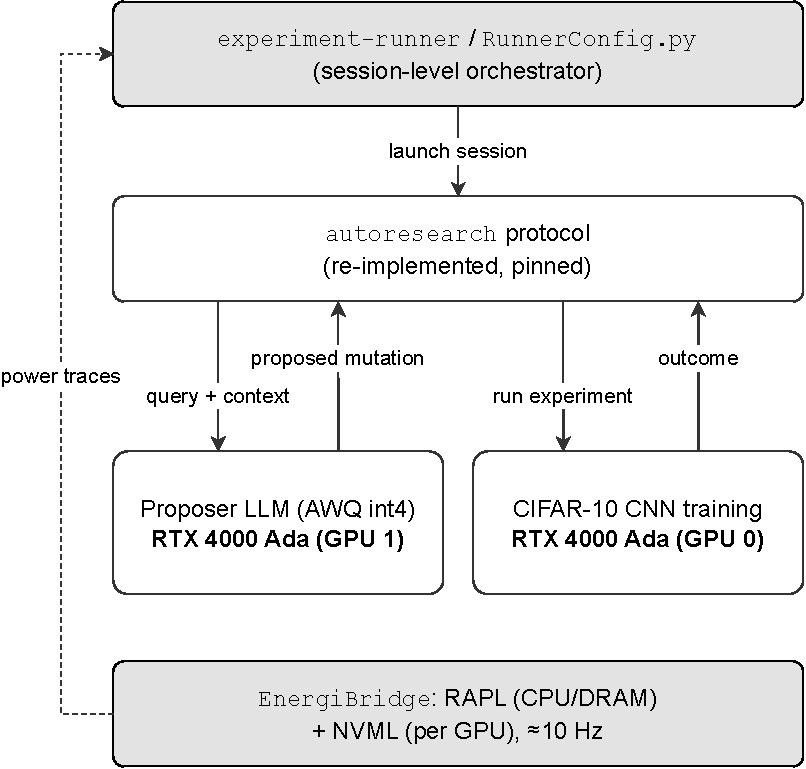
\includegraphics[width=\columnwidth]{figures/infra.drawio.pdf}
\caption{Measurement infrastructure: session-level orchestration over the agent loop, with per-GPU board measurement and phase-aligned iteration attribution.}
\Description{Architecture diagram showing experiment-runner launching the agent loop, which exchanges proposals with a Qwen model on GPU 1 and runs CIFAR-10 training on GPU 0, while EnergiBridge and NVML record energy traces.}
\label{fig:infra}
\end{figure}

\textbf{Executed procedure.} Calibration set the inner training budget to 45\,s: the reference recipe left $+15.27$\,pp of headroom above baseline, compared with $+14.32$\,pp at 240\,s, while signal-to-noise differed by only 8\,\%. Eight baseline repeats with a 120\,s cool-down gave a detrended standard deviation of 0.62\,pp, from which the keep threshold $\epsilon=0.0123$ was derived. The 24-session Phase-1 factorial then ran with randomized, interleaved cells; the completed reasoning and temperature follow-ups added 30 sessions. All 54 campaign sessions are valid. The planned eight-session CPU-served proposer subset was not launched while supervisor feedback is pending. The recorded GPU idle rates are retained only as contextual observations because their raw traces and a CPU-idle measurement are unavailable; they do not enter a correction.

\section{Results}\label{sec:results}

All 24 Phase-1 sessions completed and were valid: no session exceeded the 25\,\%
infrastructure-error threshold, and none was quarantined. Reported energies are
NVML per-device integrals; accuracy is CIFAR-10 test-set accuracy measured once
per session on the best recipe the agent retained.

\subsection{Descriptive results}

\begin{table}[htbp]
\centering
\caption{Phase-1 session outcomes by proposer architecture ($n=12$ each).}
\label{tab:headline}
\begin{tabular}{lrrr}
\toprule
& dense 14B & MoE 30B-A3B & change \\
\midrule
Session GPU energy (kJ)      & 156.4 & \textbf{90.7} & $-42.0\,\%$ \\
Proposer energy (kJ)         &  94.3 & \textbf{35.7} & $-62.2\,\%$ \\
Training energy (kJ)         &  62.1 & 55.0 & $-11.4\,\%$ \\
Wasted energy (kJ)           & 126.1 & 67.0 & $-46.9\,\%$ \\
Test accuracy                & 0.7939 & \textbf{0.8224} & $+2.85$\,pp \\
Kept mutations (total)       & 12 & \textbf{17} & $+42\,\%$ \\
Sessions with zero kept      & 5/12 & 1/12 &, \\
Proposal latency (s)         & 61.8 & 31.9 & $-48.4\,\%$ \\
Session wall-clock (s)       & 1515 & 1023 & $-32.5\,\%$ \\
\bottomrule
\end{tabular}
\end{table}

\begin{figure}[htbp]
\centering
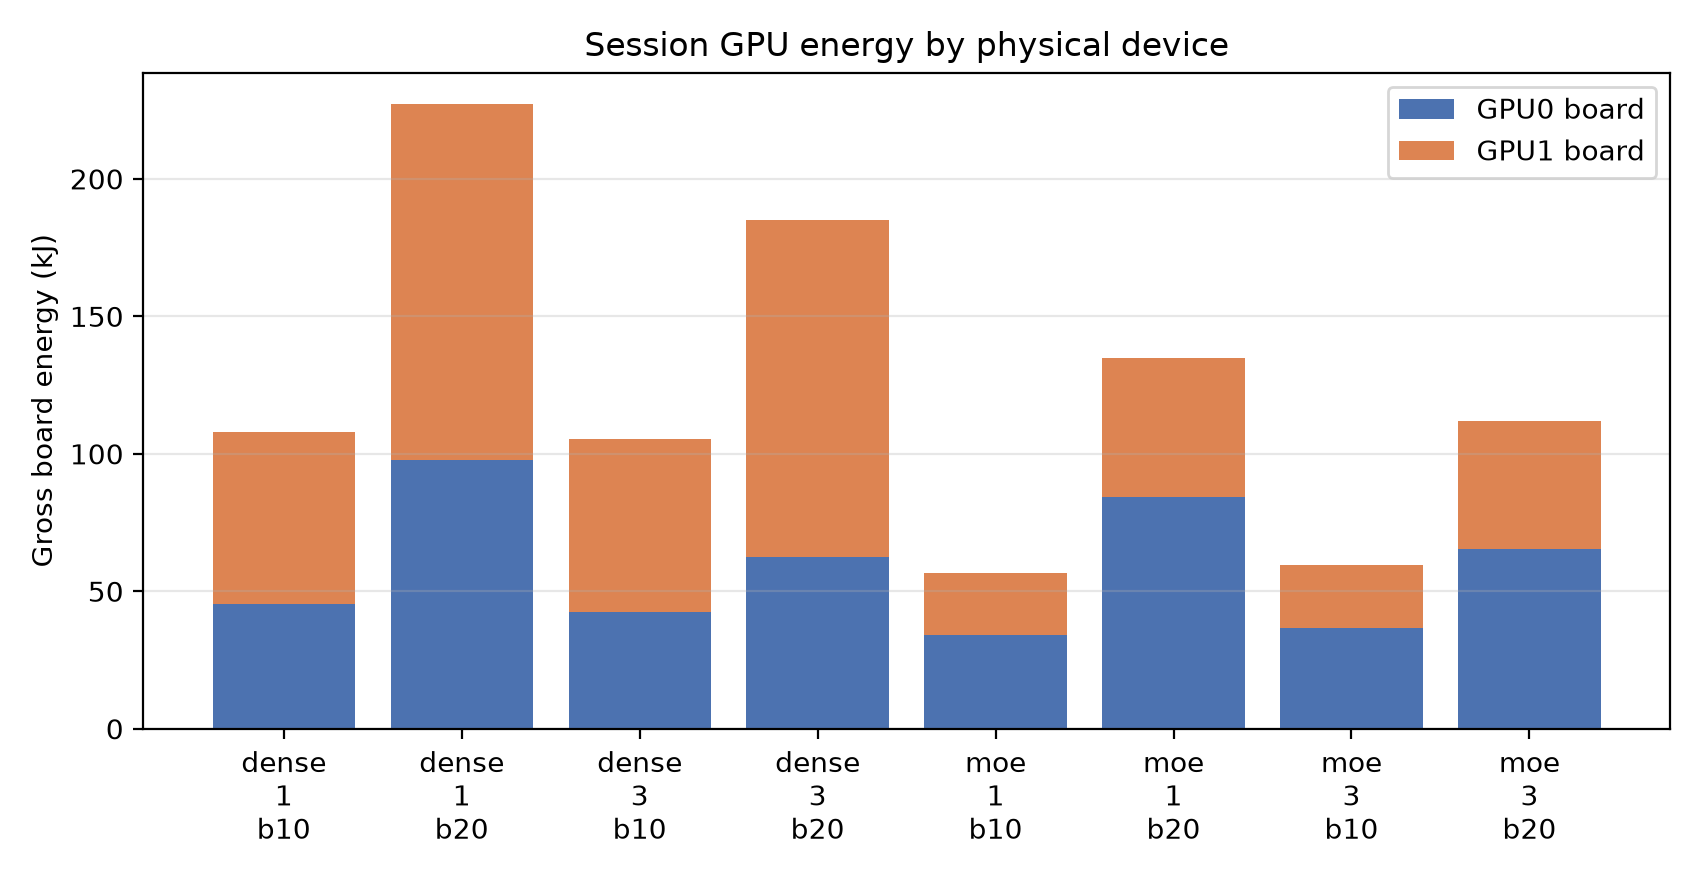
\includegraphics[width=\columnwidth]{figures/fig2_decomposition.png}
\caption{Session energy decomposed by physical device, per configuration cell.
Training energy (blue, GPU~0) is common to both arms and varies only with loop
budget; the architectural difference is concentrated almost entirely in proposer
energy (orange, GPU~1). This decomposition is a direct measurement, not an
estimate: the two components are read from separate devices.}
\label{fig:decomposition}
\end{figure}

Table~\ref{tab:headline} states the principal result: \textbf{the sparse proposer
is cheaper on every energy measure and more accurate}.
Figure~\ref{fig:decomposition} shows where the difference lives: the training
component is essentially identical across arms, as it must be, and the entire
architectural effect sits in the proposer component. This is not a trade-off
along a frontier; the MoE dominates. The mechanism is multiplicative: activating
$\sim$3B rather than 14.8B parameters draws $\sim$36\,\% less instantaneous power
(72.5\,W vs.\ 112.8\,W measured during proposal phases) \emph{and} completes a
proposal in half the time.

\begin{figure*}[htbp]
\centering
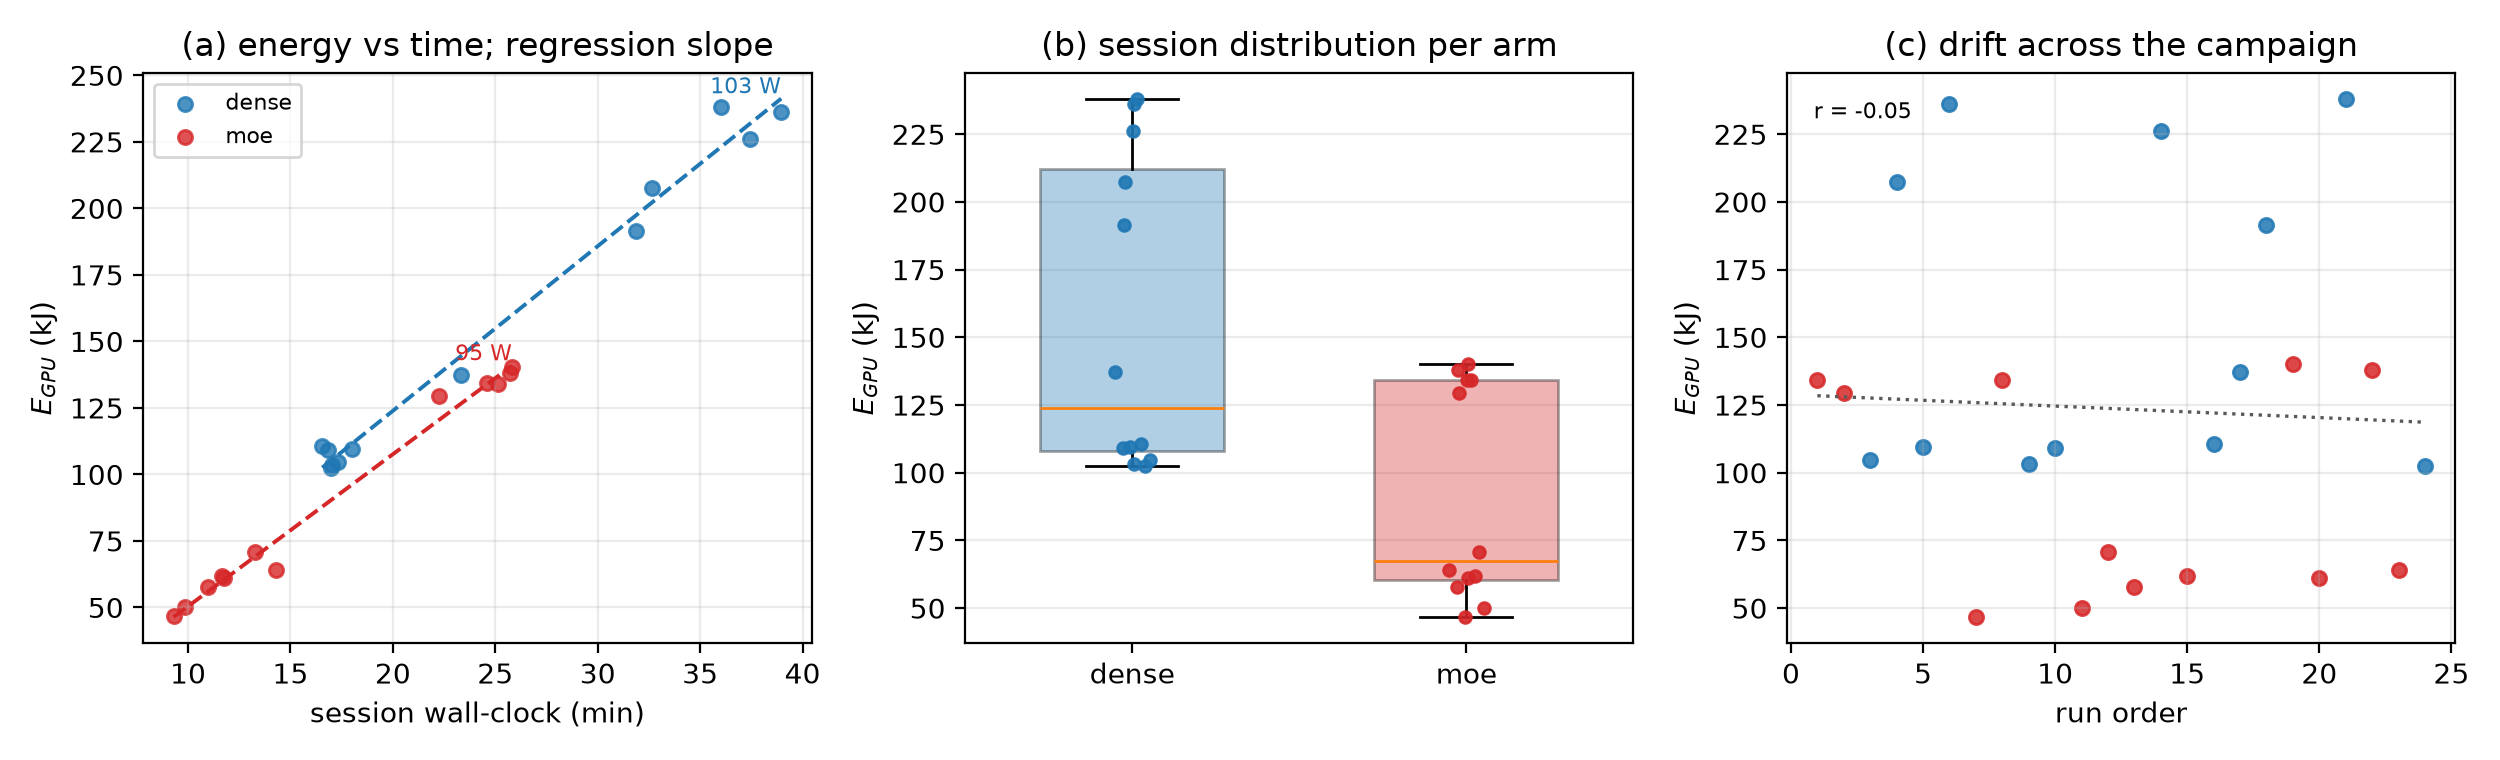
\includegraphics[width=\textwidth]{figures/fig6_diagnostics.png}
\caption{Measurement diagnostics. (a) Session energy against wall-clock; the
fitted slope is mean session power. (b) Session-level distributions per arm.
(c) Session energy against position in the randomised run table.}
\label{fig:diagnostics}
\end{figure*}

\textbf{Is this simply a speed result?} Figure~\ref{fig:diagnostics}(a) separates
the two components. Mean \emph{session} power differs by only 16\,\% between the
arms (103\,W dense, 95\,W MoE) because both share an identically loaded training
GPU; session duration differs by 48\,\%. The energy ratio decomposes as
$1.48 \times 1.16 = 1.72$, i.e.\ roughly two thirds of the session-level
advantage is shorter sessions and one third is lower power. The large power
difference is real but confined to the component the architecture governs: during
proposal phases the devices draw 112.8\,W (dense) against 72.5\,W (MoE), and
$E_{\mathit{prop}}$ per proposal differs by $2.7\times$. Reporting only session
energy would understate the architectural effect; reporting only proposer power
would overstate it.

Figure~\ref{fig:diagnostics}(c) addresses run order: energy correlates with
position in the run table at $r = -0.05$, so no thermal or environmental drift
accumulated across the campaign that randomisation would have needed to absorb.

\subsection{RQ1: effects of configuration on the energy/accuracy profile}

Shapiro--Wilk rejected normality for session energy ($W=0.889$, $p=0.012$) while
Levene's test found homoscedasticity ($p=0.46$), so the Aligned Rank Transform
was applied before ANOVA.

\begin{table}[htbp]
\centering
\caption{ART-ANOVA on session GPU energy.}
\label{tab:anova}
\begin{tabular}{lrrr}
\toprule
Effect & $F$ & $p$ & partial $\eta^2$ \\
\midrule
Proposer            & 42.61 & $6.96\times10^{-6}$ & \textbf{0.727} \\
Loop budget         & 50.58 & $2.47\times10^{-6}$ & \textbf{0.760} \\
Patience            &  2.77 & 0.116 & 0.147 \\
Proposer $\times$ patience     & 0.70 & 0.416 & 0.042 \\
Proposer $\times$ loop budget  & $\approx$0 & 1.000 & $\approx$0 \\
Patience $\times$ loop budget  & 1.39 & 0.256 & 0.080 \\
\bottomrule
\end{tabular}
\end{table}

\begin{table}[htbp]
\centering
\caption{Pre-registered contrasts. Mann--Whitney $U$, Cliff's $\delta$, Holm
correction over five tests.}
\label{tab:contrasts}
\begin{tabular}{llrlr}
\toprule
Hypothesis & Outcome & Change & Cliff's $\delta$ & $p_{\mathit{holm}}$ \\
\midrule
H$^{\mathit{prop}}$ & $E_{\mathit{total}}$   & $-42.0\,\%$ & 0.556 (large)      & 0.090 \\
H$^{\mathit{prop}}$ & test acc.              & $+3.6\,\%$  & $-0.444$ (medium)  & 0.207 \\
H$^{\mathit{bud}}$  & $E_{\mathit{per\,kept}}$ & $+107.6\,\%$ & $-0.802$ (large) & \textbf{0.024} \\
H$^{\mathit{pat}}$  & $E_{\mathit{wasted}}$  & $-9.8\,\%$  & 0.042 (negligible) & 1.000 \\
H$^{\mathit{pat}}$  & $E_{\mathit{per\,kept}}$ & $-9.4\,\%$ & 0.117 (negligible) & 1.000 \\
\bottomrule
\end{tabular}
\end{table}

Proposer architecture and loop budget both carry large effects on session energy
($\eta^2_p = 0.73$ and $0.76$); patience does not, and no interaction is
detectable. Consistent with the conclusion-validity position registered in
Section~\ref{sec:threats}, \textbf{effect sizes are the primary output}. The
architecture effect is unambiguous under ART-ANOVA ($p = 7\times10^{-6}$) while
the corresponding pairwise contrast does not survive Holm correction
($p_{\mathit{holm}} = 0.090$). These are not in conflict: the ANOVA models loop
budget, itself a large energy effect, whereas the pairwise test pools across it
and inherits that variance. With $n=12$ per arm the defensible claim is a large
and consistent effect that the corrected pairwise test is underpowered to certify
at $\alpha = 0.05$.

Doubling the loop budget from 10 to 20 raised energy per kept mutation by
$107.6\,\%$ ($\delta = -0.80$, the only Holm-significant contrast): twice the
experiments cost twice the energy per useful result, because the cheap
improvements are found early in a session.

\begin{figure}[htbp]
\centering
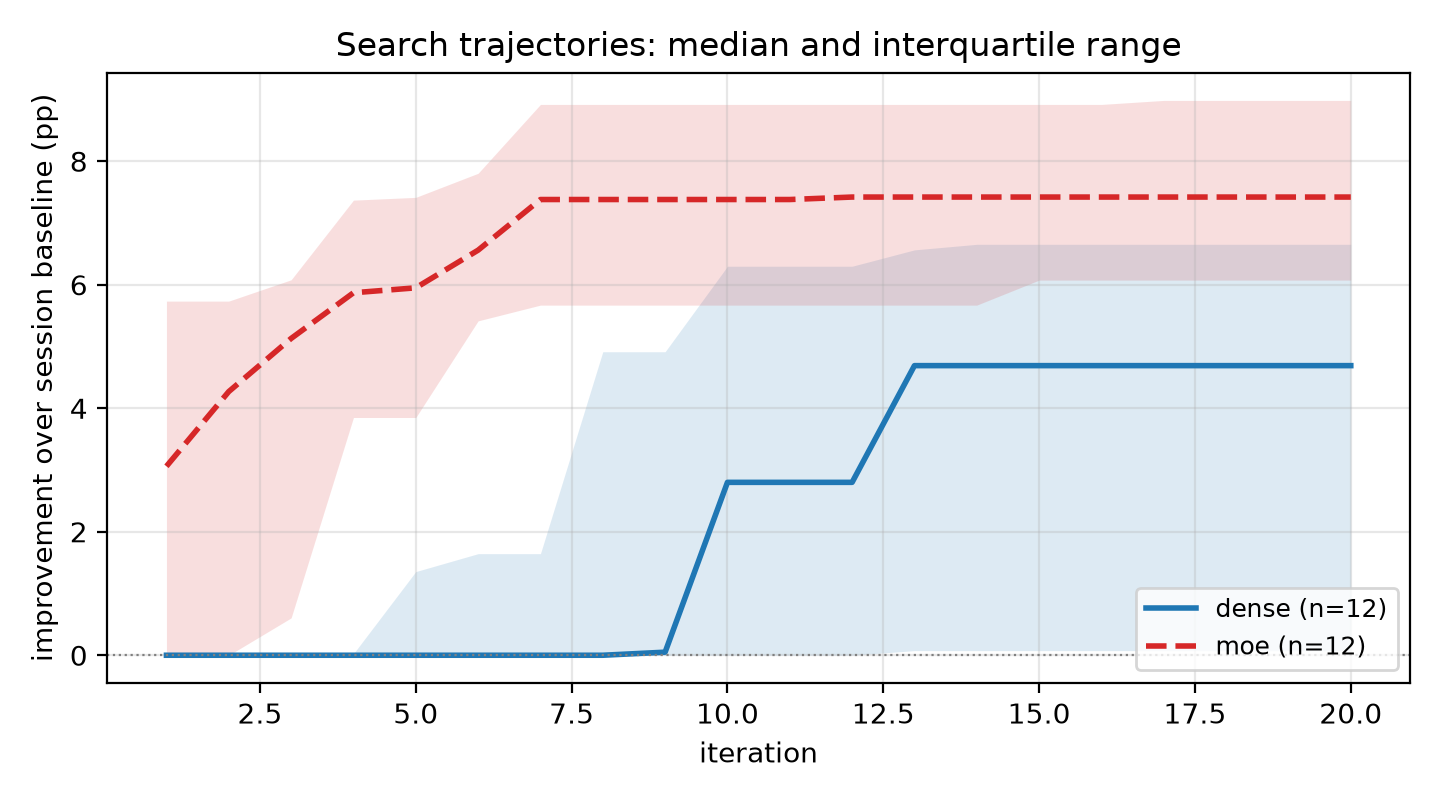
\includegraphics[width=\columnwidth]{figures/fig5_trajectories.png}
\caption{Improvement over each session's own baseline, median with
interquartile band, $n=12$ sessions per arm. Curves are monotone by
construction: a proposal that fails to improve is reverted. The MoE reaches
$+3$\,pp by its first iteration and plateaus near $+7.4$\,pp by iteration~7; the
dense arm's median is flat until iteration~9 and plateaus lower.}
\label{fig:trajectories}
\end{figure}

Figure~\ref{fig:trajectories} shows the mechanism directly, and adds a
distinction the aggregate tables cannot: the two arms differ not only in how much
they improve but in \emph{when}. The MoE's median session has gained $+3$\,pp
after a single iteration and has essentially finished by iteration~7, whereas the
dense median does not move until iteration~9. Sessions reach their final recipe
early and spend the remaining iterations proposing alternatives that are
rejected; that energy is not recovered.

\begin{figure}[htbp]
\centering
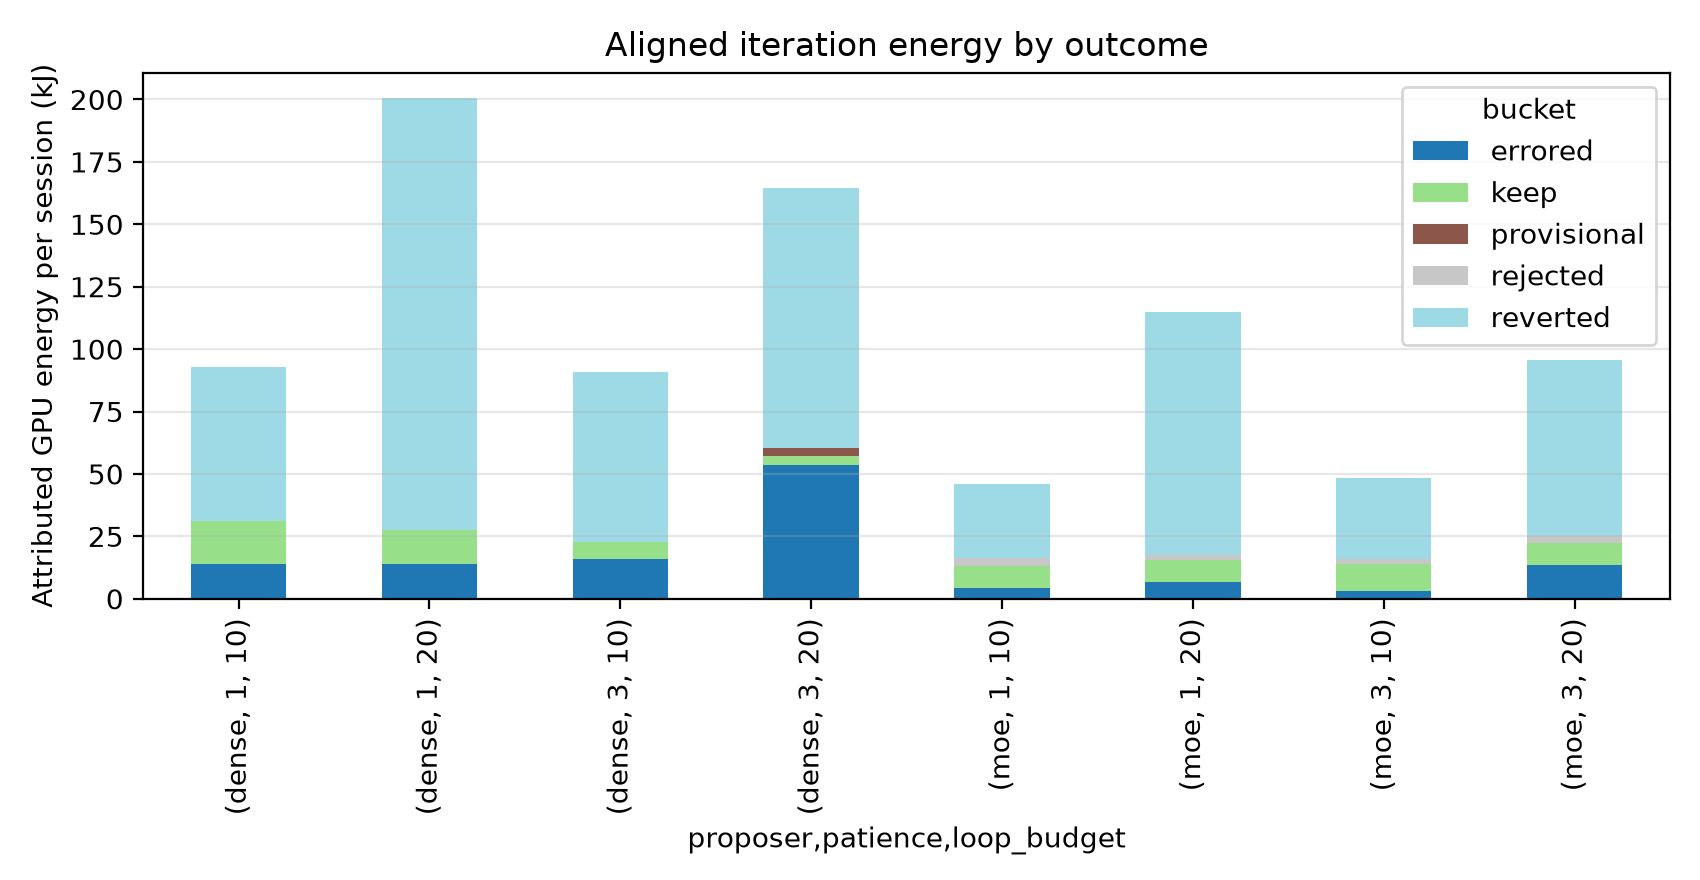
\includegraphics[width=\columnwidth]{figures/fig4_waste.png}
\caption{Per-session energy attributed to each iteration outcome. The
\emph{keep} band is small in every cell: 64\,\% of Phase-1 session energy went to
mutations that were reverted or that failed to run. This is a property of the
protocol rather than a defect, a search must evaluate candidates to
reject them, and it is precisely what makes proposer efficiency worth
measuring.}
\label{fig:waste}
\end{figure}

Figure~\ref{fig:waste} attributes that energy by outcome. Across Phase~1,
\textbf{64\,\% of session energy produced no retained mutation}, and the dense
arm wasted 126.1\,kJ per session against the MoE's 67.0\,kJ.

\subsection{RQ2: the energy/accuracy Pareto frontier}

\begin{table}[htbp]
\centering
\caption{Cell means and the non-dominated frontier.}
\label{tab:pareto}
\begin{tabular}{llrrrc}
\toprule
Proposer & Pat. & Bud. & $E$ (kJ) & Test acc. & Frontier \\
\midrule
MoE   & 1 & 10 & \textbf{56.5} & 0.8209 & yes \\
MoE   & 3 & 10 & 59.5 & 0.8134 & \\
dense & 3 & 10 & 105.4 & 0.7729 & \\
dense & 1 & 10 & 107.9 & 0.8214 & yes$^\dagger$ \\
MoE   & 3 & 20 & 112.0 & \textbf{0.8311} & yes \\
MoE   & 1 & 20 & 134.7 & 0.8242 & \\
dense & 3 & 20 & 185.0 & 0.7763 & \\
dense & 1 & 20 & 227.3 & 0.8049 & \\
\bottomrule
\end{tabular}
\end{table}

\begin{figure}[htbp]
\centering
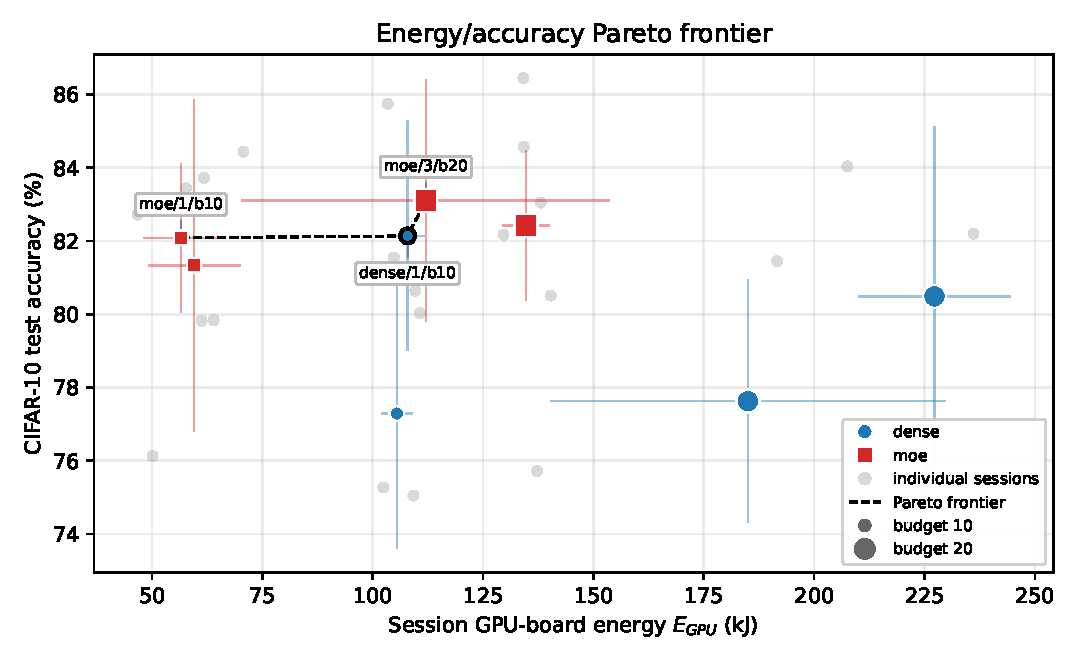
\includegraphics[width=\columnwidth]{figures/fig1_pareto.pdf}
\caption{Energy/accuracy Pareto frontier. Large markers are cell means with
$\pm$1\,SD bars; small grey points are individual sessions. Marker shape encodes
proposer, colour encodes patience, size encodes loop budget, and the designated
baseline cell (dense, greedy, budget~10) is outlined. The within-cell spread is
substantial relative to the between-cell differences in accuracy, which is why
frontier membership is interpreted against the measured noise floor rather than
from means alone.}
\label{fig:pareto}
\end{figure}

Two of the three non-dominated cells are MoE cells, and the cheapest frontier
point (MoE, greedy, budget 10) attains 0.8209 test accuracy for 56.5\,kJ,
\textbf{47.6\,\% less energy than the designated baseline cell} (dense, greedy,
budget~10) at 0.05\,pp lower mean accuracy, i.e.\ at no measurable accuracy cost., 
Figure~\ref{fig:pareto} also makes the dispersion visible: within-cell spread is
large relative to between-cell accuracy differences, which is the reason the
frontier is read against the noise floor below.

\textbf{The dense frontier point ($\dagger$) is an artifact of measurement noise
and should not be read as a genuine trade-off.} It is non-dominated only because
its mean accuracy exceeds the cheapest MoE cell by $0.053$\,pp, 23 times
smaller than the measured keep threshold ($\epsilon = 1.23$\,pp,
Section~\ref{sec:execution}) and 60 times smaller than the within-cell standard
deviation ($3.1$\,pp), while consuming $1.91\times$ the energy. A frontier
computed from cell means without reference to the noise floor will report
spurious non-dominated points; we therefore report each frontier margin against
$\epsilon$.

\subsection{Reliability of improvement}

\begin{table}[htbp]
\centering
\caption{Best accuracy \emph{observed} within a session, relative to that
session's own baseline (retained regardless of the keep decision).}
\label{tab:reliability}
\begin{tabular}{lrr}
\toprule
& Mean & Median \\
\midrule
dense 14B    & $-2.21$\,pp & $+4.69$\,pp \\
MoE 30B-A3B  & $+7.23$\,pp & $+7.42$\,pp \\
\bottomrule
\end{tabular}
\end{table}

The dense arm's mean is negative while its median is positive: a minority of
sessions collapse catastrophically, individual proposals reached $0.0924$
validation accuracy, chance level for ten classes, and pull the mean below
baseline. The MoE's mean and median nearly coincide.

\textbf{The architectural difference is therefore one of reliability as much as
of quality.} For a self-hoster this is the more consequential property: a session
that ends below its own baseline has spent its entire energy budget for a
negative result. We report best-observed accuracy alongside best-kept accuracy
because the latter collapses to the baseline whenever no proposal clears
$\epsilon$, and carries no signal in those sessions.

\subsection{Energy per kept mutation: reporting convention}

$E_{\mathit{per\,kept}}$ is undefined for a session that keeps nothing, and 5 of
12 dense sessions kept nothing (against 1 of 12 for the MoE; Fisher exact
$p=0.155$). The choice of convention materially changes the reported effect:

\begin{table}[htbp]
\centering
\caption{Two conventions for energy per kept mutation.}
\label{tab:perkept}
\small
\begin{tabular}{lrrr}
\toprule
Convention & dense & MoE & ratio \\
\midrule
Mean of ratios$^\dagger$ & 112.1\,kJ & 74.4\,kJ & $1.51\times$ \\
Pooled $\sum E / \sum \mathit{kept}$ & \textbf{156.4}\,kJ & \textbf{64.0}\,kJ & $\mathbf{2.44\times}$ \\
\bottomrule
\end{tabular}
\par\smallskip
{\footnotesize $^\dagger$ mean of the per-session ratios, which necessarily
excludes sessions that kept nothing.}
\end{table}

The first convention understates the effect by 38\,\% precisely because it
discards the sessions in which the dense arm performed worst. We report the
pooled figure and state the zero-kept counts alongside it.

\subsection{Agent behaviour}

\textbf{Contract compliance and proposal quality are independent axes.} The
guard rejected 0.0\,\% of dense proposals and 9.6\,\% of MoE proposals (maximum
30\,\% in one session), yet the MoE produced the better recipes. A benchmark
scoring only output-format compliance would rank these two models in the opposite
order. The same dissociation appeared in the pilot, where a 4B model was rejected
on four of six iterations and still gained $+8.8$\,pp while a 14B model complied
perfectly and gained nothing.

\textbf{Failure to run is a dependent variable.} Sessions averaged 4.1 (dense) and
3.3 (MoE) crashed proposals, with single-session extremes of 19/20 and 15/20.
Because a crashed proposal consumes a full proposer inference and returns
nothing, crash rate feeds directly into energy efficiency. A representative
failure: the dense proposer replaced
\texttt{SGD} at \texttt{lr=0.01} with \texttt{AdamW} at the same rate, retaining a
learning rate roughly an order of magnitude too large for Adam, and reached
$0.0924$ accuracy.

\textbf{Thinking mode was verified, not assumed.} Summing reasoning tokens over
all 360 proposals in both arms yields zero, confirming that
\texttt{enable\_thinking:\,false} was honoured by the serving stack rather than
merely accepted.

\subsection{Stage 2a: does reasoning pay for itself?}\label{sec:results:reasoning}

Reasoning mode is a fixed variable in Stage~1 (disabled for both arms, verified
at zero tokens across all 360 Phase-1 proposals). Stage~2a promotes it to a
factor: \texttt{proposer} $\times$ \texttt{thinking}, 3 repetitions, greedy,
budget~10. All 12 sessions were valid. The manipulation is confirmed by
measurement rather than by configuration: every \texttt{off} session emitted
exactly 0 reasoning tokens and every \texttt{on} session between 23\,909 and
47\,904.

\begin{table}[htbp]
\centering
\caption{Stage 2a cells ($n=3$ each).}
\label{tab:reasoning}
\begin{tabular}{llrrrrr}
\toprule
Arm & Think & $E$ (kJ) & $E_{\mathit{prop}}$ & Test acc. & Kept & Err. \\
\midrule
dense & off & 108.1 & 59.2  & 0.7572 & 0.33 & 1.0 \\
dense & on  & 172.6 & 133.3 & 0.8490 & 1.33 & 4.3 \\
MoE   & off & \textbf{52.1} & \textbf{22.0} & 0.8469 & \textbf{2.00} & 3.3 \\
MoE   & on  & 92.0  & 59.0  & 0.8378 & 1.00 & 4.3 \\
\bottomrule
\end{tabular}
\end{table}

\begin{figure}[htbp]
\centering
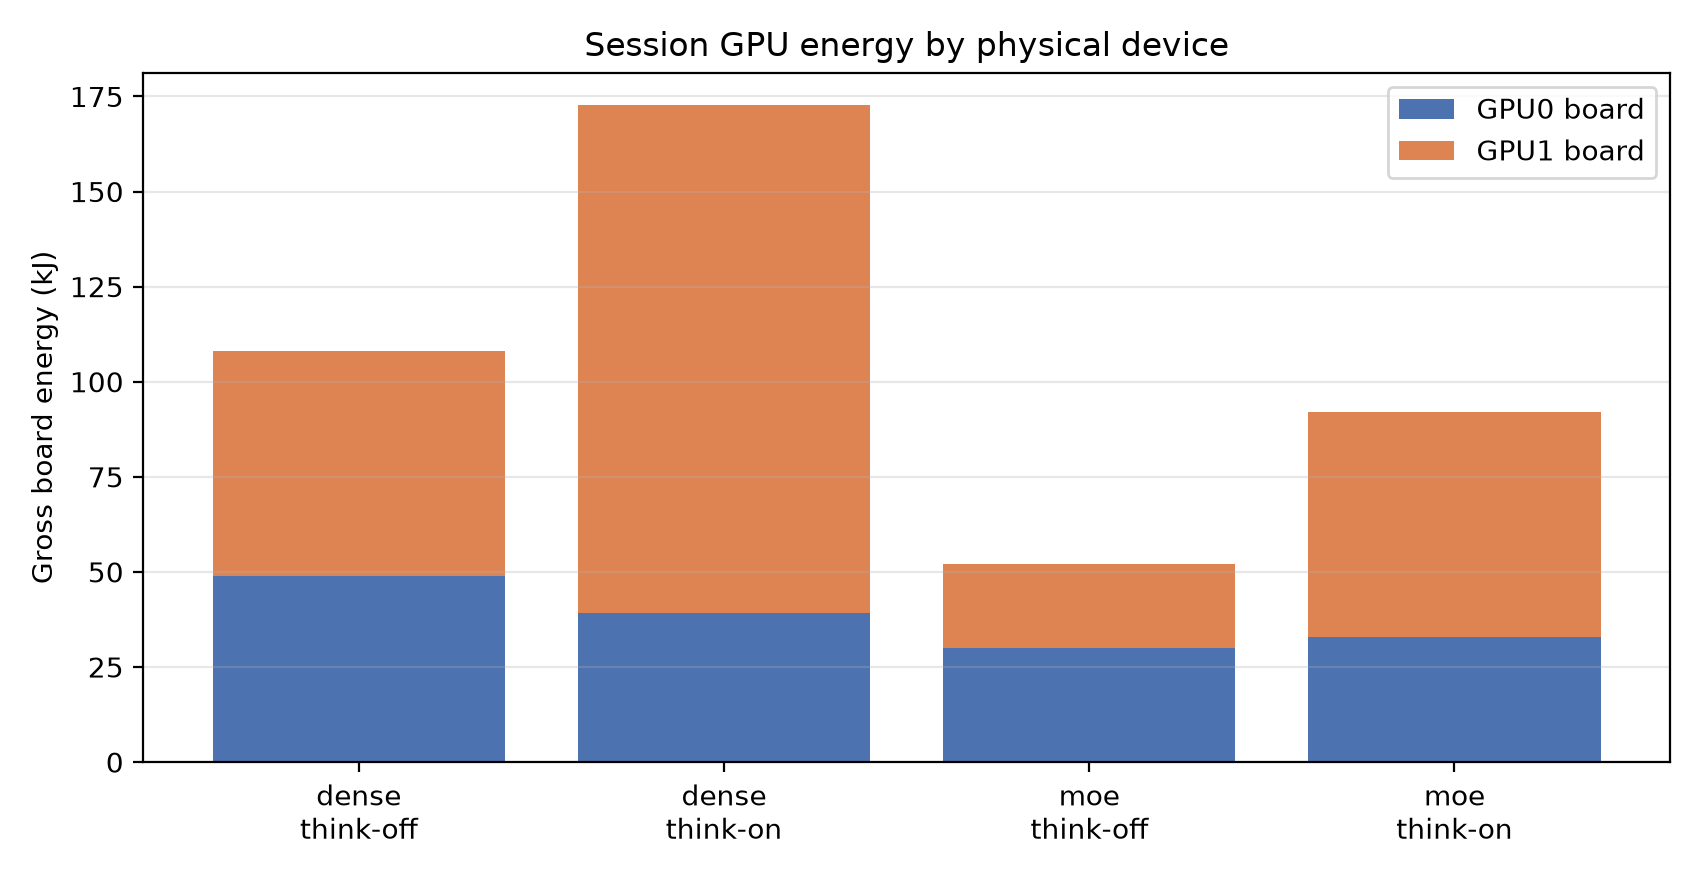
\includegraphics[width=\columnwidth]{figures/fig3_reasoning_decomposition.png}
\caption{Stage 2a: session energy by device. Reasoning inflates the proposer
component (orange) while leaving training (blue) unchanged, as it must. The two
configurations that matter are the extremes: \emph{MoE without reasoning} at
52\,kJ and \emph{dense with reasoning} at 173\,kJ, which reach statistically
indistinguishable accuracy.}
\label{fig:reasoning}
\end{figure}

\textbf{Reasoning and sparsity are substitutes, not complements.} Enabling
reasoning raises dense test accuracy substantially but leaves the MoE unchanged:
the MoE difference of $0.91$\,pp lies below the measured keep threshold
($\epsilon = 1.23$\,pp) and is not interpretable as an effect. Pooling the two
independent executions of the dense-without-reasoning configuration
(Section~\ref{sec:results:control}, $n=6$) puts the dense gain at $+6.0$\,pp.

\textbf{The practitioner reading inverts the intuitive one.} The cheapest
configuration measured, MoE without reasoning, attains 0.8469 test accuracy for
52.1\,kJ, against dense with reasoning at 0.8490 for 172.6\,kJ: \textbf{3.3
times less energy for an accuracy difference of 0.21\,pp}, six times smaller than
the noise floor. On a fixed energy budget, sparsity is the efficient purchase and
reasoning tokens are not; reasoning is an expensive route to a point the sparse
model reaches without it.

We registered a quantitative prediction before running, derived from the
feasibility probe and the measured proposal-phase power draws: that the MoE could
reason for less energy than the dense model spends not reasoning (6.17 vs.\
6.73\,kJ per proposal). The direction held and the absolute values fell within
5\,\% of prediction (5.90 vs.\ 5.92\,kJ), but the margin collapsed from 0.56 to
0.02\,kJ. The defensible claim is equality, not inequality.

Finally, reasoning did \emph{not} reduce coding errors: failures per session rose
in both arms (dense 1.0~$\rightarrow$~4.3, MoE 3.3~$\rightarrow$~4.3). We had
expected a reasoning pass to catch errors such as retaining an SGD learning rate
when switching to AdamW. It did not; longer deliberation produced more ambitious
proposals rather than more correct ones.

\subsection{A reproducibility control}\label{sec:results:control}

Phase~1's \emph{dense, greedy, budget-10} cell and Stage~2a's \emph{dense,
reasoning-off} cell are the same configuration, executed in independent
experiments days apart on the same hardware. They therefore function as an
unplanned replication.

\begin{table}[htbp]
\centering
\caption{The same configuration, executed twice independently.}
\label{tab:control}
\begin{tabular}{lrrl}
\toprule
& Phase 1 & Stage 2a & Agreement \\
\midrule
Session energy & 107.9\,kJ & 108.1\,kJ & \textbf{0.20\,\%} \\
Test accuracy  & 0.8214 & 0.7572 & 6.42\,pp apart \\
Kept mutations & 1.67 & 0.33 &, \\
\bottomrule
\end{tabular}
\end{table}

\textbf{Energy reproduces to a fifth of a percent; accuracy does not reproduce at
$n=3$.} The measurement apparatus is thus not the source of the accuracy
variance; the agent is. This is the clearest available justification for the
conclusion-validity position registered in Section~\ref{sec:threats}, that effect
sizes rather than significance tests are the primary output, and it is a concrete
warning against reading any individual three-session cell as a point estimate of
accuracy. It also implies that the energy comparisons in this study are
considerably better powered than the accuracy comparisons and should carry
correspondingly more of the argument.

\subsection{Stage 2b: sampling temperature, and a correction}\label{sec:results:temperature}

Phase~1 was restarted once because its first three sessions kept no mutations at
all, which we attributed at the time to sampling temperature 0 making the search
degenerate. Stage~2b tests that attribution directly: four temperatures, three
repetitions, MoE arm, against the current prompt.

\begin{table}[htbp]
\centering
\caption{Stage 2b: sampling temperature, MoE arm ($n=3$ per level).}
\label{tab:temperature}
\small
\begin{tabular}{rrrrrr}
\toprule
$T$ & $E$ (kJ) & Test acc. & Kept & Duplicate pairs & Distinct \\
\midrule
0.0 & 65.8 & 0.8289 & 1.67 & 23 & 0.77 \\
0.4 & 65.6 & 0.8222 & 1.67 & 5  & 0.90 \\
0.7 & 55.4 & 0.8137 & 1.33 & 2  & 0.97 \\
1.0 & 66.0 & 0.8173 & 2.33 & 9  & 0.87 \\
\bottomrule
\end{tabular}
\end{table}

\textbf{Temperature changes proposal duplication but not outcomes.} Byte-identical
proposal pairs fall from 23 at $T=0$ to between 2 and 9 above it, and the fraction
of distinct proposals within a session rises from 0.77 to 0.97. Retained
mutations (1.33--2.33) and best observed accuracy (0.8235--0.8361) show no
corresponding pattern. One $T=0$ session produced only 4 distinct proposals out of
10 and still retained 2 mutations, reaching 0.8486. Duplicate proposals waste
iterations; on this evidence they do not prevent a session from succeeding.

\textbf{The original attribution was wrong.} At $T=0$ against the current prompt
the MoE retains 1.67 mutations per session, which is the normal rate for that
arm. Temperature 0 therefore does not produce sessions that retain nothing, and
cannot by itself explain the restarted Phase~1.

Two other findings account for what we saw. First, the three sessions that
prompted the restart were, by the shuffled run order, all dense
($P = 0.11$ for the first three runs of a balanced 24-row table). Second, the
dense arm retains nothing in 5 of its 12 Phase-1 sessions even at $T=0.7$ with
the corrected prompt, a rate of 0.42. Three consecutive zero-retention dense
sessions is therefore an ordinary draw rather than evidence of a broken search.

\textbf{What the prompt did.} The restart also added a measured statement of the
training budget to the prompt. That change is not neutral, but its effect is
arm-specific: of the dense arm's \texttt{T\_max} literals in Stage 2a, 19 of 20
still specify more than 60 epochs for a budget that delivers roughly 43, whereas
the MoE emits none out of 82 in Stage 2b. The dense proposer continues to design
for a training run it is not given, after being told what it is given.

\textbf{Limits of this correction.} Stage 2b varies temperature on the MoE only,
so we have not tested $T=0$ on the dense arm against the corrected prompt. What
we can state is that the mechanism we proposed does not operate on the arm we
tested, that temperature has no detectable effect on any outcome over $[0, 1]$,
and that the observation which triggered the restart is adequately explained
without it.

\section{Discussion}\label{sec:discussion}

\subsection{RQ1: what the factor effects mean}

\textbf{The energy result is stronger than the accuracy result.} The MoE uses
42.0\,\% less GPU-board energy per session, and the broader recovered scope
(both GPU boards plus AMD CPU-package energy) still shows a 39.0\,\% reduction.
The latter is a measured-component sensitivity, not full-system energy: the trace
contains no DRAM, board, storage, fan, or power-supply losses. Mean test accuracy
is 2.85\,pp higher for the MoE, but its 95\,\% interval includes zero and the HC3
sensitivity is also nonsignificant. The defensible conclusion is therefore a
large energy advantage with no observed mean-accuracy penalty, not established
accuracy superiority or statistical equivalence.

The mechanism is multiplicative. During proposal windows the MoE device draws
72.5 rather than 112.8\,W and mean proposal latency is roughly half as long.
Whole-session GPU~1 energy is 62.2\,\% lower. GPU~0 session energy also differs
by 11.4\,\% because a board-level counter includes idle time while the proposer
runs; it is not a pure training-phase integral. This distinction matters: separate
devices support direct attribution, but labels such as ``proposer energy'' and
``training energy'' are too strong for their whole-session totals.

The fixed 10- and 20-iteration budgets also narrow the causal claim. A better
proposer cannot reduce the planned number of experiments in this harness; it
changes how many useful mutations those joules produce. The study therefore
demonstrates \emph{energy productivity} (energy per retained improvement), not a
feedback mechanism in which poor steering automatically schedules more training.
A success- or patience-based stopping design would be needed to test that latter
mechanism.

Correctly pooling all sessions, including the six with no retained improvement,
gives 156.4\,kJ/keep for dense and 64.0\,kJ/keep for MoE ($-59.1\,\%$). Five dense
sessions and one MoE session made no retained progress (Fisher $p=0.155$); keep/
revert semantics restore the starting recipe in those cases, so they did not end
below baseline. Candidate quality is nevertheless less stable for dense: its
best evaluated candidate remained below the starting validation baseline in
3/12 sessions, against 0/12 for MoE.

\textbf{Loop budget has diminishing energy productivity.} The original analysis
averaged only defined per-session ratios and silently dropped zero-kept sessions.
The corrected ratio of pooled sums is 61.8 vs.\ 152.1\,kJ/keep for budgets 10 and
20, an increase of 146.2\,\% (bootstrap ratio CI $[1.29,4.46]$). Patience changes
the pooled value by $+24.3\,\%$, not the previously reported $-9.4\,\%$, and its
wide interval includes both directions. These corrections leave the budget
conclusion intact and make the patience conclusion explicitly uncertain.

\subsection{RQ2: reading the frontier}

Two of three sample non-dominated cells are MoE cells, and the cheapest is MoE,
greedy, budget 10 at 56.5\,kJ and 0.8209 mean test accuracy. Energy dominance is
clear; the exact accuracy ordering is not. The dense frontier cell exceeds that
cell by only 0.053\,pp at $1.91\times$ the energy, while the high-budget MoE cell
adds 1.02\,pp at $1.98\times$ the energy. Both accuracy margins are below the
1.23\,pp validation keep threshold, but this threshold measures within-session
re-run noise and is not an equivalence margin for independent test-set means.
Consequently the frontier is practitioner-relevant as a sample summary, with
accuracy membership treated as provisional.

\subsection{Reasoning and temperature follow-ups}

Stage~2a provides exploratory evidence of an architecture--reasoning
interaction. Reasoning changes dense accuracy by $+9.18$\,pp and MoE accuracy by
$-0.91$\,pp; the HC3 interaction is $-10.09$\,pp. Reasoning raises proposer-device
energy in both arms, and the MoE/off cell uses 52.1\,kJ against 172.6\,kJ for
dense-with-reasoning. Their observed accuracies differ by only 0.21\,pp, but the
95\,\% interval ($[-3.97,4.38]$\,pp) is far too wide to establish equivalence.
At $n=3$ per cell, ``reasoning substitutes for sparsity'' is a useful hypothesis
for replication, not a settled generalization.

Stages~2b and 2c establish a narrower temperature result: exact duplicate
proposals are more common at $T=0$ on both arms. They do not establish that
temperature has no effect on retention or accuracy. Each level has only three
sessions, and the Phase-1 restart changed temperature and prompt content together.
The $T=0$ sessions under the current prompt show that deterministic sampling is
not sufficient to force zero retention; they cannot rule out a temperature-by-
prompt interaction. This is why the original diagnosis is reported as unsupported
rather than ``refuted'' in a causal sense.

\subsection{The harness is part of the instrument}

The prompt supplied facts the agent could not otherwise observe (tensor layout,
library versions, and the number of epochs a 45\,s budget permits). Each changed
agent behavior without changing executable workload code. The restart episode
shows why such interventions must change one factor at a time and why early rows
of a randomized run table should not be treated as representative.

An unplanned, functionally equivalent dense/off control occurred in Phase~1 and
Stage~2a. The proposer token cap differed (8,192 vs.\ 12,288) but was non-binding;
session GPU energy agrees to 0.20\,\%, while mean test accuracy differs by
6.42\,pp. Energy measurement is therefore much more stable than the agent-side
accuracy outcome at three repetitions. Follow-ups should allocate more repetitions
to fewer accuracy comparisons.

\subsection{Contract compliance is not proposal quality}

The guard rejected none of the dense proposals and 9.6\,\% of the MoE proposals,
yet the MoE produced the better observed recipes. The pilot showed the same
dissociation. Output-format compliance and proposal quality should therefore be
reported as separate axes rather than combined into one agent score.

\section{Threats To Validity}\label{sec:threats}

\subsection{Internal Validity}
\emph{Run order and thermal drift}: cell order is randomized and interleaved across the run table, with a \textbf{120\,s} inter-session cool-down. The pilot showed this is not cosmetic: eight baseline repeats without a cool-down gave a standard deviation of 1.01\,pp, and the same measurement with a cool-down gave 0.37\,pp. Across Phase~1, GPU energy correlates with position in the run table at $r=-0.05$. \emph{Background load}: sessions ran on a dedicated workstation. \emph{Idle draw}: the notes retain GPU rates of 8.63 and 7.90\,W, but neither the idle traces nor a CPU-idle measurement survive. No baseline subtraction is performed; gross energy is the auditable outcome.

\emph{Sampling temperature, and a diagnosis we had to retract.} An earlier draft
fixed proposer sampling at temperature 0 for determinism. Phase~1's first three
sessions retained no mutations at all, and we attributed this to a degenerate
search: with greedy selection the recipe returns to the baseline after every
rejection, so the prompt barely changes between iterations and a deterministic
proposer returns a nearly unchanged answer. We changed sampling to $T=0.7$,
$\mathit{top\text{-}p}$ 0.95, discarded those sessions and restarted.

Stages 2b and 2c (Sections~\ref{sec:results:temperature}
and~\ref{sec:results:dense-temp}) show that $T=0$ is not sufficient to force zero
retention under the current prompt. Temperature changes duplication (MoE 23
duplicate pairs at $T=0$ against 2--9 above it; dense 9 against 0), but three
sessions per level provide no outcome-effect estimate. Because the restart also
changed prompt content, a temperature-by-prompt interaction remains unresolved.
The observation that triggered the restart is explained without any such
mechanism: the three sessions were all dense by the shuffled run order
($P = 0.11$), and the dense arm retains nothing in 42\,\% of its sessions even at
$T=0.7$.

We report this rather than quietly adopting the corrected account, because the
episode is itself a threat to internal validity of a kind that is easy to leave
undocumented. A mid-experiment intervention was made on a diagnosis formed from
three sessions, and it bundled two changes (sampling and prompt content) whose
effects could not afterwards be separated without a further experiment. The
sessions discarded at that point were valid measurements. Our practice for the
remainder of the study was to change one thing at a time and to record the
intervention as data.

\emph{The prompt is part of the instrument.} Three times the experiment was floored by information the agent could not observe rather than by any property of the models: the data contract (that \texttt{load\_splits()} returns pre-normalised NCHW tensors) reduced crashes from 4 in 5 iterations to 1 in 5; the library versions in the execution environment reduced them from 7 in 9 to 0 in 10; and stating what the wall-clock budget actually buys ($\approx$43 epochs) stopped the agent proposing schedules written for hundreds. Each correction was comment-only, changing no executable line, so the calibration results remained valid. The principle applied throughout was to \textbf{supply facts the agent cannot observe and withhold the judgement under measurement}: tensor shapes and library versions are properties of the environment a human collaborator would simply read, whereas ``retune the learning rate when changing optimiser'' is the reasoning being evaluated. An under-specified prompt produces a floor effect that is indistinguishable, in the results, from poor model capability.

\subsection{External Validity}
Results are conditional on one workload (a compact CIFAR-10 CNN at a 45\,s budget), one model family (Qwen3), one quantization method and level (AWQ int4), and one hardware configuration. A vision CNN also exercises the training GPU differently from the LLM-training workload \texttt{autoresearch} was built around (shorter kernels, lower memory pressure), so per-session energy profiles will not transfer directly to \texttt{nanochat}-style workloads. The MoE-vs-dense contrast generalizes only to the extent that Qwen3's sparsity design is representative of self-hostable MoE models.

Two properties of the subject pair bound the claim further. \emph{Publisher asymmetry}: no single publisher ships AWQ builds of both models, so the dense arm uses Qwen's official quantization and the MoE a third-party build. The method and bit-width are identical; the calibration corpus is not. \emph{Unequal total capacity} (30.5B vs.\ 14.8B): sparsity and capacity cannot be fully separated, so the study answers ``which architecture is more efficient per joule on one 20\,GB card'' and not ``is sparsity superior at matched capacity''. The latter required Qwen3-32B, which does not fit.

\emph{Compiled kernels}: attention kernels are JIT-compiled for the local architecture (sm89) against a pinned stack (vLLM 0.27.1, FlashInfer 0.6.16.post3, torch 2.13.0, CUDA 13.0, driver 580.159.03). Absolute joules are specific to this stack and silicon; both arms share one build, so the contrast is unaffected. \emph{Prefix caching} is enabled, as it is by default in production serving, so from the second iteration the shared prompt prefix skips prefill; this is realistic and identical across arms, but per-iteration proposer energy is not uniform within a session. The \texttt{nanochat} workload is specified as the first extension, and broader workload generalization is out of scope.

\subsection{Construct Validity}
\emph{Energy scope and attribution}: separate GPUs provide direct board readings, but whole-session totals include idle and model-residency draw and are not pure training/proposer components. The registered pipeline omitted the AMD \texttt{CPU\_ENERGY} column because it expected Intel-style labels; post-hoc counter reconstruction is therefore reported separately. GPU+CPU-package energy still omits DRAM and uninstrumented host components. Iteration accounting leaves a 13.6\,\% unaligned remainder. The implemented alignment flag accepted a remainder below 50\,\%, rather than the planned 1\,\% reconstruction tolerance; since ``accounted + remainder = total'' is algebraic, this flag validates only a loose coverage bound. Phase-level claims are consequently based on explicitly aligned windows and the remainder is shown separately. \emph{Accuracy} is operationalized by validation and test accuracy, kept distinct from keep/revert decisions. \emph{Short-budget scale}: eight repeats of the unmodified baseline at 45\,s give a detrended standard deviation of 0.62\,pp, hence $\epsilon=0.0123$.

\emph{Energy versus duration}: the ratio of arm-mean GPU energy to arm-mean duration is 103.2\,W for dense and 88.7\,W for MoE (16.4\,\% apart), while duration is 48\,\% apart. Separate regression slopes are 103.2 and 95.3\,W; mixing the MoE slope with the ratio-of-means decomposition would be incorrect. Proposal-window power is 112.8 vs.\ 72.5\,W. We report both duration and power rather than interpreting gross energy as an intrinsic hardware efficiency alone.

\emph{Frontier uncertainty}: a Pareto frontier computed from cell means can report non-dominated points whose accuracy advantage is tiny relative to within-cell variation. The 1.23\,pp keep threshold characterizes within-session validation re-runs; it is not an equivalence margin for between-cell test means. Frontier membership is therefore descriptive and should be reassessed with more repetitions or bootstrap dominance probabilities.

\emph{Fixed-budget mechanism}: every valid Phase-1 session exhausts 10 or 20 iterations. A stronger proposer improves retained yield but cannot reduce the scheduled training count. Claims about spending inference savings back through additional downstream experiments therefore lie outside this design; energy per retained change is the supported construct.

\emph{Undefined ratios}: $E_{\mathit{per\,kept}}$ does not exist for a session that keeps nothing, and such sessions are not evenly distributed between arms (5 of 12 dense, 1 of 12 MoE). Averaging only the defined values discards precisely the sessions in which the weaker arm performed worst and understates the effect by 38\,\%. The pooled ratio $\sum E / \sum \mathit{kept}$ is reported instead, with zero-kept counts stated alongside.

\subsection{Conclusion Validity}
The Phase-1 design is small-$N$ (8 cells $\times$ 3 repetitions): two-level factors detect only monotonic effects, and power for accuracy interactions is limited. Stage~2 cells also have three repetitions and are exploratory. Effect estimates with intervals are therefore emphasized; no-progress sessions are retained in pooled estimands. The four raw campaign archives contain traces, logs, summaries, and recipe-history bundles, but the public repository/DOI and environment manifest remain packaging work rather than completed replication claims.

\section{Reflection}\label{sec:reflection}

This section addresses the three reflective requirements of the Research Project:
the novelty of the results, their efficacy, and what I learned. I write in the
first person here because the judgements are mine.

\subsection{Novelty}

Three contributions appear to be new, in descending order of confidence.

\textbf{An energy measurement of an agentic AutoML loop for which I found no
direct precedent.} Published
inference-energy work measures single prompts \cite{luccioni2024power};
MLAgentBench \cite{huang2024mlagentbench} measures agent success rates and API
cost but not energy. In a literature search last updated in August~2026, I did
not identify a prior study that measures the energy of a directly comparable
closed propose--evaluate--keep loop. Under this experiment's fixed iteration
budgets, proposal quality determines retained yield rather than how many training
runs are scheduled. The specific finding is a large sparse-proposer energy
advantage with a higher, but statistically uncertain, mean accuracy; it is one
workload and one model pair.

\textbf{Per-device energy attribution as a design choice rather than a model.}
Placing proposer inference and inner-loop training on physically separate GPUs
means GPU~1 and GPU~0 board energy are read from different devices rather than
separated by a calibration model. Whole-session device totals still include idle
and residency energy. Phase-aligned power checks confirm that GPU~0 draws more
during training and GPU~1 during proposing; the looser reconstruction flag itself
is only a coverage check and should not be mistaken for a 1\,\% accuracy test.

\textbf{A methodological result that generalises beyond these subjects.} A keep
threshold must be derived from a measured noise floor; the value I specified
a~priori sat four times below it, at which point ``retained mutation'' is not a
meaningful event. I consider this more portable than the architectural result,
because it applies to any study of this loop shape.

I had intended to claim a second one, that deterministic sampling makes such a
loop degenerate. The follow-up showed that $T=0$ is not sufficient to cause this
under the revised prompt. What
survives is narrower: temperature governs how often the proposer repeats itself.
The available outcome samples do not establish a null effect on retention or
accuracy.

I am less confident about novelty in one respect. The observation that contract
compliance and proposal quality are independent axes is, I suspect, known
informally to practitioners; my contribution is a measurement of it
(0.0\,\% vs.\ 9.6\,\% guard-rejection rates, with the more-rejected arm producing
better recipes) rather than the observation itself.

\subsection{Efficacy: what worked and what did not}

\textbf{What worked.} Calibrating before measuring was decisive. The training
budget, keep threshold and cool-down were each set from measurement, and each
differed materially from the value I had assumed, the budget by a factor of
five, the threshold by a factor of twelve. Had I run the factorial on the assumed
values, the keep/revert decision would have been noise and the study would have
produced a clean-looking null.

The gate structure also worked, in an unglamorous way: gate G1 rejected the
originally proposed model pair on arithmetic before 44\,GB had been downloaded a
second time, and the alignment gate would have caught crossed device indices had
there been any.

\textbf{What did not.} I diagnosed a broken experiment from its first three
sessions and acted on it. Those sessions retained no mutations, I concluded that
sampling at temperature 0 had made the search degenerate, and I changed
temperature and restarted. The reasoning was plausible and the supporting
evidence was real: the proposals were 0.982 similar on average with one pair
identical. It was still overconfident. Later sweeps on both arms showed that
temperature 0 can retain mutations under the revised prompt, and that three
sessions retaining nothing is plausible for the dense arm, which retains nothing
in 42\,\% of its Phase~1 sessions. The
run order is randomised precisely so that the first few runs are not
representative, and I read them as though they were.

I compounded it by changing two things at once. The restart altered sampling and
added the budget facts to the prompt, so even after the sweep I can only say that
temperature 0 is not sufficient under the revised prompt, not what either change contributed on the
dense arm. Eighteen sessions were spent recovering an answer that a
one-change-at-a-time intervention would have given for free.

I also under-powered accuracy relative to energy. An unplanned, functionally
equivalent control (the proposer token caps differed but were non-binding),
executed in two experiments days apart, reproduced GPU-board session energy to
0.20\,\% and test accuracy to only 6.42\,pp. Given that
variance structure, spending the same machine time on more repetitions of fewer
cells would have produced tighter accuracy estimates. I would make that trade
differently if I repeated this.

\subsection{What I learned}

\textbf{An agentic harness is a measuring instrument, and its prompt is part of
the instrument.} Three times the experiment was floored not by any property of
the models but by information the agent could not observe: that the data was
already normalised, that the installed library versions had removed the APIs it
was using, and how few epochs the wall-clock budget actually buys. Each fix was
comment-only and each moved the crash rate substantially. The line I settled on,
supply facts the agent cannot observe and withhold the judgement being measured,
is one I would now apply from the start rather than derive under pressure.

\textbf{Do not diagnose an experiment from its opening runs.} This is the
mistake I would most want to avoid repeating. Randomised run order guarantees
that early sessions are an arbitrary subset, and three of eight cells is not a
sample from which to infer a mechanism. What made it seductive was that I had a
plausible mechanism ready and evidence that fit it; what I lacked was any check
that the evidence discriminated between my explanation and a simpler one.

\textbf{Plausible output is more dangerous than failure.} The failures that cost
me the most were the ones that produced valid-looking data: a profiler faithfully
recording an idle machine because the program it was supposed to wrap had died
silently; an analysis pipeline grouping results by the wrong factor and printing
a plausible table; a run table that a hard stop had left malformed in a way that
only surfaced days later. None raised an error. I have come to trust a crash considerably more than
a clean run, and to check the content of results rather than their shape.

\textbf{Measurement infrastructure is most of the work.} The scientific question
took twenty-four sessions and about ten GPU-hours. Getting to the point where
those sessions meant anything took substantially longer, and most of the
deviations recorded in this report are infrastructural rather than conceptual. I
had not appreciated how much of empirical computer science is instrument-building
before doing it.

\textbf{Reading someone else's analysis script is cheap and worth doing.} Late in
the project I revisited the analysis template from the Green Lab course. Two of
its habits were missing from my pipeline and neither was expensive: plotting the
dependent variable against duration, and against run order. The first turned out
to matter, it separates an efficiency claim from a speed claim, and my
headline result needed that separation to be defensible. The second confirmed
that randomisation had done its job. I had built more sophisticated analysis than
the template and still omitted two of its cheapest and most useful checks, which
suggests I should read comparable work for its routine practice and not only for
its findings.

\textbf{Effect sizes over significance, understood rather than recited.} The
design pre-registered effect sizes as the primary output, which I initially
treated as a convention of the field. The replication above made it concrete:
with agent-side variance of that magnitude at $n=3$, a significance test on
accuracy answers a question about sample size rather than about proposers.

\section{Conclusions}\label{sec:conclusions}

On this agentic AutoML workload, the Qwen3 sparse proposer has a clear energy
advantage over the dense proposer. It uses 42.0\,\% less GPU-board energy per
session (90.7 vs.\ 156.4\,kJ). Reconstructing the archived AMD CPU-package
counter over the same session boundaries gives 179.8 vs.\ 294.5\,kJ, a 39.0\,\%
reduction at the broader measured-component scope. Neither quantity is idle-
subtracted, and the latter is not full-system energy because DRAM and other host
components are absent.

The MoE's mean test accuracy is 2.85\,pp higher (0.8224 vs.\ 0.7939), but its
95\,\% interval includes zero. We therefore conclude that the energy advantage is
established for this design while accuracy superiority and equivalence are not.
The MoE retained 17 improvements against 12 and had one no-progress session
against five. Correctly pooling all sessions gives 64.0 vs.\ 156.4\,kJ of GPU
energy per retained improvement ($-59.1\,\%$); adding CPU-package energy gives
126.9 vs.\ 294.5\,kJ ($-56.9\,\%$). No-progress sessions finish on the starting
recipe under keep/revert semantics, not below it.

Loop budget is the clearest agent-policy result. Raising the budget from 10 to 20
increases pooled GPU energy per retained improvement by 146.2\,\%, with a
bootstrap interval excluding no change. The corrected patience estimate changes
direction relative to the original per-session-ratio analysis and remains
uncertain. Of Phase-1 GPU energy, 78.1\,\% is attributable to non-retained
iterations, 8.2\,\% to retained iterations, and 13.6\,\% lies outside aligned
iteration windows. This is energy productivity under a fixed budget: the design
does not show that poor proposals cause the loop to schedule more training.

The sample Pareto frontier contains two MoE cells and one dense cell. The cheapest
MoE cell is the natural low-energy choice, but exact frontier membership on the
accuracy axis is provisional because cell means are noisy. The measured keep
threshold is a within-session validation rule, not a between-cell test-accuracy
equivalence margin.

The exploratory reasoning experiment suggests an architecture-by-reasoning
interaction: reasoning raises energy in both arms, improves dense accuracy in
this sample, and does not improve the MoE sample. MoE-without-reasoning reaches
nearly the same observed mean accuracy as dense-with-reasoning for roughly one
third of its GPU energy, but the accuracy interval is too wide for equivalence.
The temperature follow-ups establish that $T=0$ increases exact duplication on
both arms. They do not establish a null effect on retention or accuracy, because
each level has three sessions and the original restart changed prompt content and
temperature together.

Three extensions are now cleanly separated from completed evidence. First, a
100-iteration MoE session with post-hoc replay of every retained checkpoint is
implemented but not yet run; the manuscript will report it only after its raw
NVML and EnergiBridge traces, trajectory, and replay results are recovered.
Second, CPU-served proposer inference (with training still on GPU~0) awaits
supervisor feedback and is not part of the current conclusions. Third, wider
workload and model-family axes, including the original \texttt{nanochat} workload,
are needed before treating the observed frontier as workload-invariant.


\bibliographystyle{IEEEtran}
\bibliography{references}

\end{document}
